
%%%%%%%%%%%%%%%%%%%%%%%%%%%%%%%%%%%%%%%%
% datoteka diploma-FRI-vzorec.tex
%
%POZOR: ta verzija ne producira pdf datoteke v pdf/A formatu!!!
%namenjena je le za nalogo pri Diplomskem seminarju!
%
% vzorčna datoteka za pisanje diplomskega dela v formatu LaTeX
% na UL Fakulteti za računalništvo in informatiko
%
% na osnovi starejših verzij vkup spravil Franc Solina, maj 2021
% prvo verzijo je leta 2010 pripravil Gašper Fijavž
%
% za upravljanje z literaturo ta vezija uporablja BibLaTeX
%
% svetujemo uporabo Overleaf.com - na tej spletni implementaciji LaTeXa ta vzorec zagotovo pravilno deluje
%

\documentclass[a4paper,12pt,openright]{book}
%\documentclass[a4paper, 12pt, openright, draft]{book}  Nalogo preverite tudi z opcijo draft, ki pokaže, katere vrstice so predolge! Pozor, v draft opciji, se slike ne pokažejo!


 
\usepackage[utf8]{inputenc}   % omogoča uporabo slovenskih črk kodiranih v formatu UTF-8
\usepackage[slovene,english]{babel}    % naloži, med drugim, slovenske delilne vzorce
\usepackage[pdftex]{graphicx}  % omogoča vlaganje slik različnih formatov
\usepackage{fancyhdr}          % poskrbi, na primer, za glave strani
\usepackage{amssymb}           % dodatni matematični simboli
\usepackage{amsmath}           % eqref, npr.
\usepackage{hyperxmp}
\usepackage[hyphens]{url}
\usepackage{csquotes}
\usepackage{comment}
\usepackage[pdftex, colorlinks=true,
						citecolor=black, filecolor=black, 
						linkcolor=black, urlcolor=black,
						pdfproducer={LaTeX}, pdfcreator={LaTeX}]{hyperref}

\usepackage{color}
\usepackage{soul}

\usepackage[
backend=biber,
style=numeric,
sorting=nty,
]{biblatex}
\usepackage{blkarray,bigstrut}

\addbibresource{literatura.bib} %Imports bibliography file


%%%%%%%%%%%%%%%%%%%%%%%%%%%%%%%%%%%%%%%%
%	DIPLOMA INFO
%%%%%%%%%%%%%%%%%%%%%%%%%%%%%%%%%%%%%%%%
\newcommand{\ttitle}{Uporaba diskretne kosinusne transformacije pri kompresiji signalov}
\newcommand{\ttitleEn}{Diploma thesis template}
\newcommand{\tsubject}{\ttitle}
\newcommand{\tsubjectEn}{\ttitleEn}
\newcommand{\tauthor}{Gregor Šraj}
\newcommand{\tkeywords}{Diskretna kosinusna transformacija, JPEG}
\newcommand{\tkeywordsEn}{Discrete cosine transform, JPEG}

%%%%%%%%%%%%%%%%%%%%%%%%%%%%%%%%%%%%%%%%
%	HYPERREF SETUP
%%%%%%%%%%%%%%%%%%%%%%%%%%%%%%%%%%%%%%%%
\hypersetup{pdftitle={\ttitle}}
\hypersetup{pdfsubject=\ttitleEn}
\hypersetup{pdfauthor={\tauthor}}
\hypersetup{pdfkeywords=\tkeywordsEn}

%%%%%%%%%%%%%%%%%%%%%%%%%%%%%%%%%%%%%%%%
% postavitev strani
%%%%%%%%%%%%%%%%%%%%%%%%%%%%%%%%%%%%%%%%  

\addtolength{\marginparwidth}{-20pt} % robovi za tisk
\addtolength{\oddsidemargin}{40pt}
\addtolength{\evensidemargin}{-40pt}

\renewcommand{\baselinestretch}{1.3} % ustrezen razmik med vrsticami
\setlength{\headheight}{15pt}        % potreben prostor na vrhu
\renewcommand{\chaptermark}[1]%
{\markboth{\MakeUppercase{\thechapter.\ #1}}{}} \renewcommand{\sectionmark}[1]%
{\markright{\MakeUppercase{\thesection.\ #1}}} \renewcommand{\headrulewidth}{0.5pt} \renewcommand{\footrulewidth}{0pt}
\fancyhf{}
\fancyhead[LE,RO]{\sl \thepage} 
%\fancyhead[LO]{\sl \rightmark} \fancyhead[RE]{\sl \leftmark}
\fancyhead[RE]{\sc \tauthor}              % dodal Solina
\fancyhead[LO]{\sc Diplomska naloga}     % dodal Solina


\newcommand{\BibLaTeX}{{\sc Bib}\LaTeX}
\newcommand{\BibTeX}{{\sc Bib}\TeX}

%%%%%%%%%%%%%%%%%%%%%%%%%%%%%%%%%%%%%%%%
% naslovi
%%%%%%%%%%%%%%%%%%%%%%%%%%%%%%%%%%%%%%%%  

\newcommand{\autfont}{\Large}
\newcommand{\titfont}{\LARGE\bf}
\newcommand{\clearemptydoublepage}{\newpage{\pagestyle{empty}\cleardoublepage}}
\setcounter{tocdepth}{1}	      % globina kazala

%%%%%%%%%%%%%%%%%%%%%%%%%%%%%%%%%%%%%%%%
% konstrukti
%%%%%%%%%%%%%%%%%%%%%%%%%%%%%%%%%%%%%%%%  
\newtheorem{izrek}{Izrek}[chapter]
\newtheorem{trditev}{Trditev}[izrek]
\newenvironment{dokaz}{\emph{Dokaz.}\ }{\hspace{\fill}{$\Box$}}


%%%%%%%%%%%%%%%%%%%%%%%%%%%%%%%%%%%%%%%%%%%%%%%%%%%%%%%%%%%%%%%%%%%%%%%%%%%%%%%
%% PDF-A
%%%%%%%%%%%%%%%%%%%%%%%%%%%%%%%%%%%%%%%%%%%%%%%%%%%%%%%%%%%%%%%%%%%%%%%%%%%%%%%

%%%%%%%%%%%%%%%%%%%%%%%%%%%%%%%%%%%%%%%% 
% define medatata
%%%%%%%%%%%%%%%%%%%%%%%%%%%%%%%%%%%%%%%% 
\def\Title{\ttitle}
\def\Author{\tauthor, matjaz.kralj@fri.uni-lj.si}
\def\Subject{\ttitleEn}
\def\Keywords{\tkeywordsEn}

%%%%%%%%%%%%%%%%%%%%%%%%%%%%%%%%%%%%%%%% 
% \convertDate converts D:20080419103507+02'00' to 2008-04-19T10:35:07+02:00
%%%%%%%%%%%%%%%%%%%%%%%%%%%%%%%%%%%%%%%% 
\def\convertDate{%
    \getYear
}

{\catcode`\D=12
 \gdef\getYear D:#1#2#3#4{\edef\xYear{#1#2#3#4}\getMonth}
}
\def\getMonth#1#2{\edef\xMonth{#1#2}\getDay}
\def\getDay#1#2{\edef\xDay{#1#2}\getHour}
\def\getHour#1#2{\edef\xHour{#1#2}\getMin}
\def\getMin#1#2{\edef\xMin{#1#2}\getSec}
\def\getSec#1#2{\edef\xSec{#1#2}\getTZh}
\def\getTZh +#1#2{\edef\xTZh{#1#2}\getTZm}
\def\getTZm '#1#2'{%
    \edef\xTZm{#1#2}%
    \edef\convDate{\xYear-\xMonth-\xDay T\xHour:\xMin:\xSec+\xTZh:\xTZm}%
}

%\expandafter\convertDate\pdfcreationdate 

%%%%%%%%%%%%%%%%%%%%%%%%%%%%%%%%%%%%%%%%
% get pdftex version string
%%%%%%%%%%%%%%%%%%%%%%%%%%%%%%%%%%%%%%%% 
\newcount\countA
\countA=\pdftexversion
\advance \countA by -100
\def\pdftexVersionStr{pdfTeX-1.\the\countA.\pdftexrevision}


%%%%%%%%%%%%%%%%%%%%%%%%%%%%%%%%%%%%%%%%
% XMP data
%%%%%%%%%%%%%%%%%%%%%%%%%%%%%%%%%%%%%%%%  
\usepackage{xmpincl}
%\includexmp{pdfa-1b}

%%%%%%%%%%%%%%%%%%%%%%%%%%%%%%%%%%%%%%%%
% pdfInfo
%%%%%%%%%%%%%%%%%%%%%%%%%%%%%%%%%%%%%%%%  
\pdfinfo{%
    /Title    (\ttitle)
    /Author   (\tauthor, damjan@cvetan.si)
    /Subject  (\ttitleEn)
    /Keywords (\tkeywordsEn)
    /ModDate  (\pdfcreationdate)
    /Trapped  /False
}

%%%%%%%%%%%%%%%%%%%%%%%%%%%%%%%%%%%%%%%%
% znaki za copyright stran
%%%%%%%%%%%%%%%%%%%%%%%%%%%%%%%%%%%%%%%%  

\newcommand{\CcImageCc}[1]{%
	
\includegraphics[scale=#1]{slike/cc_cc_30.pdf}%
}
\newcommand{\CcImageBy}[1]{%
	
\includegraphics[scale=#1]{slike/cc_by_30.pdf}%
}
\newcommand{\CcImageSa}[1]{%
	
\includegraphics[scale=#1]{slike/cc_sa_30.pdf}%
}

\newcommand{\RNum}[1]{\uppercase\expandafter{\romannumeral #1\relax}}
%%%%%%%%%%%%%%%%%%%%%%%%%%%%%%%%%%%%%%%%%%%%%%%%%%%%%%%%%%%%%%%%%%%%%%%%%%%%%%%
%%%%%%%%%%%%%%%%%%%%%%%%%%%%%%%%%%%%%%%%%%%%%%%%%%%%%%%%%%%%%%%%%%%%%%%%%%%%%%%

\begin{document}
\selectlanguage{slovene}
\frontmatter
\setcounter{page}{1} %
\renewcommand{\thepage}{}       % preprečimo težave s številkami strani v kazalu

%%%%%%%%%%%%%%%%%%%%%%%%%%%%%%%%%%%%%%%%
%naslovnica
 \thispagestyle{empty}%
   \begin{center}
    {\large\sc Univerza v Ljubljani\\%
%      Fakulteta za elektrotehniko\\% za študijski program Multimedija
%      Fakulteta za upravo\\% za študijski program Upravna informatika
      Fakulteta za računalništvo in informatiko\\%
      Fakulteta za matematiko in fiziko\\% za študijski program Računalništvo in matematika
     }
    \vskip 10em%
    {\autfont \tauthor\par}%
    {\titfont \ttitle \par}%
    {\vskip 3em \textsc{DIPLOMSKO DELO\\[5mm]         % dodal Solina za ostale študijske programe
%    VISOKOŠOLSKI STROKOVNI ŠTUDIJSKI PROGRAM\\ PRVE STOPNJE\\ RAČUNALNIŠTVO IN INFORMATIKA}\par}%
%     UNIVERZITETNI  ŠTUDIJSKI PROGRAM\\ PRVE STOPNJE\\ RAČUNALNIŠTVO IN INFORMATIKA}\par}%
%    INTERDISCIPLINARNI UNIVERZITETNI\\ ŠTUDIJSKI PROGRAM PRVE STOPNJE\\ MULTIMEDIJA}\par}%
%    INTERDISCIPLINARNI UNIVERZITETNI\\ ŠTUDIJSKI PROGRAM PRVE STOPNJE\\ UPRAVNA INFORMATIKA}\par}%
    INTERDISCIPLINARNI UNIVERZITETNI\\ ŠTUDIJSKI PROGRAM PRVE STOPNJE\\ RAČUNALNIŠTVO IN MATEMATIKA}\par}%
    \vfill\null%
% izberite pravi habilitacijski naziv mentorja!
    {\large \textsc{Mentor}: doc. dr. Tadej Kanduč\par}%
    {\vskip 2em \large Ljubljana, 2023 \par}%
\end{center}
% prazna stran
\clearemptydoublepage      
% izjava o licencah itd. se izpiše na hrbtni strani naslovnice

%%%%%%%%%%%%%%%%%%%%%%%%%%%%%%%%%%%%%%%%
%copyright stran
%%%%%%%%%%%%%%%%%%%%%%%%%%%%%%%%%%%%%%%%
\newpage
\thispagestyle{empty}

\vspace*{5cm}
{\small \noindent
To delo je ponujeno pod licenco \textit{Creative Commons Priznanje avtorstva-Deljenje pod enakimi pogoji 2.5 Slovenija} (ali novej\v so razli\v cico).
To pomeni, da se tako besedilo, slike, grafi in druge sestavine dela kot tudi rezultati diplomskega dela lahko prosto distribuirajo,
reproducirajo, uporabljajo, priobčujejo javnosti in predelujejo, pod pogojem, da se jasno in vidno navede avtorja in naslov tega
dela in da se v primeru spremembe, preoblikovanja ali uporabe tega dela v svojem delu, lahko distribuira predelava le pod
licenco, ki je enaka tej.
Podrobnosti licence so dostopne na spletni strani \href{http://creativecommons.si}{creativecommons.si} ali na Inštitutu za
intelektualno lastnino, Streliška 1, 1000 Ljubljana.

\vspace*{1cm}
\begin{center}% 0.66 / 0.89 = 0.741573033707865
\CcImageCc{0.741573033707865}\hspace*{1ex}\CcImageBy{1}\hspace*{1ex}\CcImageSa{1}%
\end{center}
}

\vspace*{1cm}
{\small \noindent
Izvorna koda diplomskega dela, njeni rezultati in v ta namen razvita programska oprema je ponujena pod licenco GNU General Public License,
različica 3 (ali novejša). To pomeni, da se lahko prosto distribuira in/ali predeluje pod njenimi pogoji.
Podrobnosti licence so dostopne na spletni strani \url{http://www.gnu.org/licenses/}.
}

\vfill
\begin{center} 
\ \\ \vfill
{\em
Besedilo je oblikovano z urejevalnikom besedil \LaTeX.}
\end{center}

% prazna stran
\clearemptydoublepage

%%%%%%%%%%%%%%%%%%%%%%%%%%%%%%%%%%%%%%%%
% stran 3 med uvodnimi listi
\thispagestyle{empty}
\
\vfill

\bigskip
\noindent\textbf{Kandidat:} Gregor Šraj\\
\noindent\textbf{Naslov:} Uporaba diskretne kosinusne transformacije pri kompresiji signalov\\
% vstavite ustrezen naziv študijskega programa!
\noindent\textbf{Vrsta naloge:} Diplomska naloga na univerzitetnem programu prve stopnje Računalništvo in matematika \\
% izberite pravi habilitacijski naziv mentorja!
\noindent\textbf{Mentor:} doc. dr. Tadej Kanduč\\

\bigskip
\noindent\textbf{Opis:}\\
Besedilo teme diplomskega dela študent prepiše iz študijskega informacijskega sistema, kamor ga je vnesel mentor. 
V nekaj stavkih bo opisal, kaj pričakuje od kandidatovega diplomskega dela. 
Kaj so cilji, kakšne metode naj uporabi, morda bo zapisal tudi ključno literaturo.

\bigskip
\noindent\textbf{Title:} Naslov diplomskega dela v angleščini

\bigskip
\noindent\textbf{Description:}\\
opis diplome v angleščini

\vfill



\vspace{2cm}

% prazna stran
\clearemptydoublepage

% zahvala
\thispagestyle{empty}\mbox{}\vfill\null\it%
\noindent
Na tem mestu zapišite, komu se zahvaljujete za pomoč pri izdelavi diplomske naloge oziroma pri vašem študiju nasploh. Pazite, da ne boste koga pozabili. Utegnil vam bo zameriti. Temu se da izogniti tako, da celotno zahvalo izpustite.
\rm\normalfont


% prazna stran
\clearemptydoublepage

%%%%%%%%%%%%%%%%%%%%%%%%%%%%%%%%%%%%%%%%
% kazalo
\pagestyle{empty}
\def\thepage{}% preprečimo težave s številkami strani v kazalu
\tableofcontents{}


% prazna stran
\clearemptydoublepage

%%%%%%%%%%%%%%%%%%%%%%%%%%%%%%%%%%%%%%%%
% seznam kratic

\chapter*{Seznam uporabljenih kratic}

\noindent\begin{tabular}{p{0.11\textwidth}|p{.39\textwidth}|p{.39\textwidth}}    % po potrebi razširi prvo kolono tabele na račun drugih dveh!
  {\bf kratica} & {\bf angleško}                              & {\bf slovensko} \\ \hline
  {\bf DCT}      & Discrete cosine transform               & Diskretna kosinusna transformacija \\
  {\bf FCT}      & Fourier cosine transform               & Fourierova kosinusna transformacija \\
\end{tabular}


% prazna stran
\clearemptydoublepage
%%%%%%%%%%%%%%%%%%%%%%%%%%%%%%%%%%%%%%%%
% povzetek
\addcontentsline{toc}{chapter}{Povzetek}
\chapter*{Povzetek}

\noindent\textbf{Naslov:} \ttitle
\bigskip

\noindent\textbf{Avtor:} \tauthor
\bigskip

%\noindent\textbf{Povzetek:} 
\noindent 
V tem diplomskem delu smo pokazali kako je definirana diskretna kosinusna transformacija in tudi idejo njene izpeljave. Pokazali smo kako se razširi ta definicija na dve dimenzije in da lahko dvodimenzionalno obliko izračunamo s pomočjo enodimenzionalne. Opisali smo primer algoritma za hiter izračun DCT s pomočjo že obstoječih algoritmov FFT. Podobno smo opisali primer algoritma Integer DCT, ki teče na bolj enostavni aritmetiki. Poglobili smo se v delovanje najbolj pogoste implementacije JPEG. Tu smo opisali celoten postopek, kako se blok originalne slike zakodira v bitni niz, ki se shrani in pošilja. Opisali smo potek obratnega procesa dekodiranja. Nato smo na primeru dejanskega bloka prikazali kako ta postopek poteka. Za konec smo nekaj dejanskih slik pretvorili v JPEG format z različnimi nivoji kvalitete. Izračunali smo PSNR teh slik in primerjali kateri nivoji kvalitete so primerni za različne aplikacije. 

\bigskip

\noindent\textbf{Ključne besede:} \tkeywords.
% prazna stran
\clearemptydoublepage
%%%%%%%%%%%%%%%%%%%%%%%%%%%%%%%%%%%%%%%%
% abstract
\selectlanguage{english}
\addcontentsline{toc}{chapter}{Abstract}
\chapter*{Abstract}

\noindent\textbf{Title:} \ttitleEn
\bigskip

\noindent\textbf{Author:} \tauthor
\bigskip

%\noindent\textbf{Abstract:} 
\noindent This sample document presents an approach to typesetting your BSc thesis using \LaTeX. 
A proper abstract should contain around 100 words which makes this one way too short.
\bigskip

\noindent\textbf{Keywords:} \tkeywordsEn.
\selectlanguage{slovene}
% prazna stran
\clearemptydoublepage
%%%%%%%%%%%%%%%%%%%%%%%%%%%%%%%%%%%%%%%%
\mainmatter
\setcounter{page}{1}
\pagestyle{fancy}


\chapter{Uvod}
Diskretna kosinusna transformacija (DCT) in njej podobne metode so temelj vse današnje komunikacije preko spleta, kjer je kompresija podatkov ključna za hitro pošiljanje podatkov. Uporablja se v formatih za slike kot so JPEG, WebP, HEIF, BPG ... Pri formatih za posnetke kot so H.264, H.265, Apple ProRes, AV1 ... Pri formatih za zvočne posnetke MP3, AAC ... \par
Osredotočili se bomo na uporabo DCT pri slikah, vendar se ta ideja dokaj enostavno razširi na posnetke, saj pri njih velja še več uporabnih lastnosti. Ne samo, da so korelirani sosednji piksli, korelirani so tudi piksli na istih lokacijah v zaporednih sličicah. Podobno je ta metoda tudi uporabna za zvok.\par
Ukvarjali se bomo z uporabo DCT pri kompresiji signalov. V \ref{DCT}. poglavju bomo predstavili teoretično ozadje DCT. Najprej bomo povedali idejo izpeljave DCT. Podali bomo definicijo te metode na eni dimenziji in nato razširitev na dve dimenziji ter kako lahko z dvodimenzionalen problem pretvorimo na enodimenzionalen problem. Vizualno bomo predstavili kaj pomeni transformacija slike z DCT in kaj nam bodo predstavljali koeficienti v novem prostoru. Ideja te metode je, da obstaja med sosednjimi podatki korelacija. Te korelirane podatke želimo preslikati v nekoreliran frekvenčen prostor, kjer bomo prihranili prostor s tem, da bomo potrebovali manj podatkov za shranjevanje podatkov, kjer bomo izgubili minimalno natančnost. S to preslikamo se izgubi nekaj podatkov, saj je DCT kompresija z izgubo (\textit{angl.} lossy compression), ti podatki so tisti, ki imajo visoko frekvenco. Na ta način bomo lahko shranili sliko z manj biti, kar bo za nas predstavljalo prihranek prostora. DCT specifično je tako uporaben, ker je njegov izračun lahko implementiran na zelo hiter način. Ta lastnost je pomembna, saj je na primer pri posnetkih včasih potrebno, da kompresija poteka v realnem času. Pokazali bomo tudi metodo, ki lahko teče na bolj enostavni aritmetiki.\par
V \ref{JPEG}. poglavju se bomo osredotočili na slike, saj je na njih najenostavneje predstaviti, kako deluje DCT v praksi in kakšne prihranke nam omogoča. Specifično bomo opisali format JPEG. Pokazali bomo kako sliko preslikamo v prostor DCT in katere podatke odstranimo, da bo vizualno najmanjša razlika med originalno in skrčeno sliko. Opisali bomo tudi kodiranje, ki se uporablja v tem procesu. Ta celoten proces kodiranja bomo tudi predstavili na dejanskem primeru. Za konec bomo pa pokazali kako dekodiramo podatke nazaj v sliko.\par
V zadnjem \ref{Uporaba_DCT}. poglavju bomo na nekaj slikah pokazali kako izgledajo slike JPEG, kjer nastavimo njihove kvalitete na različne ravni. Izračunali bomo njihov PSNR in pogledali kaj to pomeni v praksi.\par



\chapter{Diskretna kosinusna transformacija} 
\label{DCT}
DCT preslika signal v prostor diskretnih baznih funkcij. To se uporablja pri kompresiji, saj so signali v tem prostoru bolj nekorelirani. Najprej bomo pokazali kako pridemo do zvezne oblike, torej Fourierove kosinusne transformacije (FCT). Nato bomo opisali idejo diskretizacije, da dobimo DCT. 
\section{Fourierova kosinusna transformacija}%vir (http://dsp-book.narod.ru/BYPRDCT.pdf)
Izpeljavo FCT bomo naredili po~\cite{britanak2010discrete} s pomočjo Fourierove transformacije. Dano imamo funkcijo $x(t)$ na intervalu $-\infty < t < \infty$. Če obstaja spodnji integral, je Fourierova transformacija funkcije $x(t)$ podana z

\begin{equation}
X(\omega) \equiv F[x(t)] = \left( \frac{1}{2 \pi} \right)^{1/2} \int\limits_{-\infty}^{\infty} x(t) e^{-i \omega t} \,dt.
\label{eq:FT}
\end{equation}

Tukaj sta $i = \sqrt{-1}$ in $\omega = 2 \pi f$ je krožna frekvenca, kjer je $f$ frekvenca v Hertzih.  Iz Fourierove transformacije lahko $x(t)$ dobimo nazaj z inverzno Fourierovo transformacijo

\begin{equation}
x(t) \equiv F^{-1}[X(\omega)] = \left( \frac{1}{2 \pi} \right)^{1/2} \int\limits_{-\infty}^{\infty} X(\omega) e^{i \omega t} \,d\omega.
\label{eq:IFT}
\end{equation}
V teh definicijah smo uporabili naslednje oznake:
\begin{itemize}
  \item $t$\ldots parameter iz fizičnega prostora
  \item $F$\ldots Fourierova transformacija
  \item $F^{-1}$\ldots inverzna Fourierova transformacija
  \item $x$\ldots funkcija iz fizičnega prostora
  \item $X$\ldots funkcija iz frekvenčnega prostora
  
\end{itemize}
Uporabljena je definicija Fourierove transformacije in inverzne Fourierove transformacije, ki ima kot vodilna faktorja $\left( \frac{1}{2 \pi} \right)^{1/2}$. Nekatere druge literature navajajo to definicijo drugače. Različne definicije tukaj privedejo do različnih definicij FCT. Tudi lastnosti Fourierove transformacije in FCT so odvisne od uporabljene definicije.\par

Če je $x(t)$ definirana samo za $t \geq 0$, lahko konstruiramo sledečo funkcijo $y(t)$:

\begin{equation}
    y(t) =
    \begin{cases}
        x(t),  & t \geq 0\\
        x(-t), & t \leq 0\\
    \end{cases}.
\end{equation}

Potem sledi:

\begin{equation}
  \begin{aligned}
    F[y(t)] & = \left( \frac{1}{2 \pi} \right)^{1/2}
              \left\{ \int\limits_{0}^{\infty} x(t) e^{-i \omega t} dt +
                  \int\limits_{-\infty}^{0} x(-t) e^{-i \omega t} dt \right\}\\
            & = \left( \frac{1}{2 \pi} \right)^{1/2}
                \int\limits_{0}^{\infty} x(t) \left[ e^{-i \omega t} + 
                                                     e^{i \omega t}\right] dt\\
            & = \left( \frac{2}{\pi} \right)^{1/2}
                \int\limits_{0}^{\infty} x(t)  \cos(\omega t) dt\\
  \end{aligned}
\label{eq:izpeljava_FCT}
\end{equation}

Zdaj lahko definiramo FCT za $x(t)$ kot

\begin{equation}
X_C(\omega) \equiv F_C[x(t)]= \left( \frac{2}{\pi} \right)^{1/2} 
                          \int\limits_{0}^{\infty} x(t)  \cos(\omega t) \,dt.
\label{eq:FCT}
\end{equation}

Če uporabimo dejstvo, da je $X_C(\omega)$ soda funkcija, lahko uporabimo Fourierov inverz na \eqref{eq:izpeljava_FCT} in dobimo

\begin{equation}
y(t) = x(t) \equiv F_C^{-1}[X_C(\omega)]= \left( \frac{2}{\pi} \right)^{1/2} 
            \int\limits_{0}^{\infty} X_C(\omega)  \cos(\omega t) \,d\omega, \indent t \geq 0.
\label{eq:Inverzni_FCT}
\end{equation}

Rezultati FCT so v realnem prostoru medtem, ko so bili rezultati Fourierove transformacije v kompleksnem prostoru.

\section{Izpeljava DCT}
DCT ni zgolj diskretizirana verzija FCT. Ta zgolj zgleda kot zvezna verzija DCT vendar to zares ne velja. DCT pride iz rešitve diferencialne enačbe s specifičnimi robnimi pogoji. Odvisno od robnih pogojev, ki jih vzamemo dobimo različne variante DCT. Ta izpeljava je opisana v~\cite{britanak2010discrete}.  Varianta, ki se najbolj uporablja in o kateri mi govorimo je DCT tipa \RNum{2}, inverzni DCT je tipa \RNum{3}. V celotni diplomski nalogi, ko se sklicujemo na DCT mislimo s tem DCT tipa \RNum{2}. 

\section{Enodimenzionalni DCT}% vir (https://web.archive.org/web/20150711105353/http://wisnet.seecs.nust.edu.pk/publications/tech_reports/DCT_TR802.pdf)
Najpogostejša definicija DCT enodimenzionalnega zaporedja dolžine N je % definicija iz članka

\begin{equation}
C(u) = \alpha(u)  \sum_{x=0}^{N-1} f(x)\cos\left[\frac{\pi(2x+1)u}{2N}\right],  \indent 
u = 0,1,2,\ldots,N-1,
\label{eq:1D-DCT}
\end{equation}
kjer je $f(x)$ realna funkcija, definirana na $x = 0,1,2,\ldots,N-1$.
Podobno je inverzna transformacija definirana kot 

\begin{equation}
f(x) = \sum_{u=0}^{N-1} \alpha(u)C(u)\cos\left[\frac{\pi(2x+1)u}{2N}\right],  \indent 
x = 0,1,2,\ldots,N-1.
\label{eq:1D-DCT-inverse}
\end{equation}

V definicijah \eqref{eq:1D-DCT} in \eqref{eq:1D-DCT-inverse} je $\alpha(u)$ definiran kot 

\begin{equation}
\alpha(u)=
    \begin{cases}
          \sqrt{\frac{1}{N}}, & u=0 \\
          \sqrt{\frac{2}{N}}, & u\neq 0 \\
    \end{cases}.
\label{eq:definicija_alpha}
\end{equation}

V definiciji DCT smo $f(x)$ v \eqref{eq:1D-DCT-inverse} zapisali v bazi kosinusnih funkcij. Torej baza DCT je $B = \{\cos\frac{\pi(2x+1)u}{2N}, \; x = 0,1,2,\ldots,N-1 \}$. To pomeni, da smo funkcijo f, ki je podana v fizičnem prostoru, običajno kot nek signal, zapisali v frekvenčnem prostoru. Vrednosti $C(u)$, nam predstavljajo utež vsake funkcije v bazi. Vrednostim $C(u)$ običajno rečemo kar koeficienti DCT.

Definirajmo še DCT v matrični obliki, saj bomo to obliko kasneje potrebovali. Naj bo $C_N$ matrika, kjer velja

\begin{equation}
[C_N]_{xu} = \left[\alpha(u) \cos\frac{\pi(2x+1)u}{2N}\right], \indent 
x,u = 0,1,2,\ldots,N-1.
\label{eq:1D_DCT_matrika}
\end{equation}

Zapišemo $f(x)$ kot vrstični vektor \(f = 
\begin{bmatrix} 
f(0) & f(1) & \ldots & f(N-1)
\end{bmatrix}.
\)
Potem lahko izračunamo \(C =  
\begin{bmatrix} 
C(0) & C(1) & \cdots & C(N-1)
\end{bmatrix}
\)
kot $C = fC_N$
Iz \eqref{eq:1D-DCT} očitno sledi 
$C(0) = \sqrt{\frac{1}{N}} \sum_{x=0}^{N-1} f(x)$. Torej je prvi transformacijski koeficient povprečna vrednost vzorčnega zaporedja. V literaturi se ta vrednost običajno imenuje DC koeficient. Vsi ostali koeficienti se imenujejo AC koeficienti. Ta imena izhajajo iz zgodovinskih razlogov, ko se je DCT uporabljal za analiziranje električnih vezij z direktnimi in izmeničnimi tokovi. \par

Povejmo še nekaj o časovni zahtevnosti tega algoritma. Imamo signal dolžine n. Želimo izračunati njegov DCT. Če računamo po definiciji \eqref{eq:1D-DCT} moramo izračunati n koeficientov DCT. Za vsakega od teh koeficientov potrebujemo n seštevanj. Za vsako od števil, ki jih seštejemo potrebujemo še prej nekaj seštevanj in množenj vendar to je za vsak posamezen koeficient $\mathcal{O}(1)$. Torej skupna računska zahtevnost je $\mathcal{O}(n^2)$. Pri inverzni DCT pridemo po podobnem postopku do istega računske zahtevnosti. \par

Za idejo kako to zgleda lahko izpustimo komponenti $f(x)$ in $\alpha(u)$ v \eqref{eq:1D-DCT}. Izris grafa  $ h(x) = \cos[\frac{\pi(2x+1)u}{2N}]$ za $N=8$ in različne vrednosti $u$ je prikazan na Sliki \ref{1D_bazne_funkcije}. V skladu s prejšnjimi opazkami je pri krivulji zgoraj levo ($u=0$) izrisana konstantna (DC) vrednost, medtem ko druge krivulje ($u=1,2,\ldots,7$) dajo krivulje z vedno višjimi frekvencami. Te krivulje se kličejo kosinusne bazne funkcije. Te bazne funkcije so ortogonalne. 
\begin{figure}[ht] % vir (https://web.archive.org/web/20150711105353/http://wisnet.seecs.nust.edu.pk/publications/tech_reports/DCT_TR802.pdf)
\begin{center}
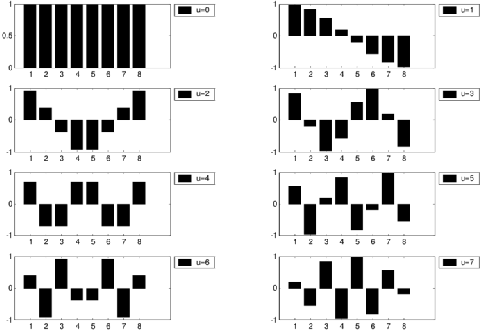
\includegraphics[width=0.8\textwidth]{slike/bazne_funkcije_1D.pdf}
\end{center}
\caption{Enodimenzionalne kosinusne bazne funkcije pri različnih $u$ ($N=8$). Na abscisi so vrednosti $x$, na ordinati so vrednosti $h(x)$. Vir:~\cite{DCT_article}.}
\label{1D_bazne_funkcije}
\end{figure}
%Iz tega sledi, da pri množenju katerekoli krivulje iz slike \ref{1D_bazne_funkcije} z drugo krivuljo in nato seštevanju preko vseh vzorčnih točk nam vrne ničelno (skalarno) vrednost. Množenje katerekoli krivulje iz slike \ref{1D_bazne_funkcije} same s sabo in nato seštevanju nam vrne konstantno (skalarno) vrednost. 

\begin{izrek}
\label{iz:dokaz_ortogonalnosti}
$C_N$ je ortogonalna matrika, torej $C_N^{-1} = C_N^T$.
\end{izrek}
\begin{dokaz}
Da se izognemo veliko trigonometrije bomo ta dokaz naredili na indirekten način.
Najprej razpišimo $C_N$;
\begin{gather}
  C_N = \sqrt{\frac{2}{N}}
  \begin{blockarray}{ccccc}
     u=0               & u= 1                                 &\dots  & u=N-1                                                  &         \\
    \begin{block}{[cccc]c}
    \frac{1}{\sqrt{2}} & \cos{(\frac{\pi}{N}\cdot \frac{1}{2})}   &\cdots & \cos{(\frac{(N-1))\pi}{N}\cdot \frac{1}{2})}\bigstrut[t]   & x=0     \\
    \frac{1}{\sqrt{2}} & \cos{(\frac{\pi}{N}\cdot \frac{3}{2})}   &\cdots & \cos{(\frac{(N-1))\pi}{N}\cdot \frac{3}{2})}               & x=1     \\
    \vdots             &\vdots                                &\ddots & \vdots                                                 &\vdots   \\
    \frac{1}{\sqrt{2}} & \cos{(\frac{\pi}{N}\cdot \frac{2N-1}{2})}&\cdots & \cos{(\frac{(N-1))\pi}{N}\cdot \frac{2N-1}{2})}\bigstrut[b]& x=N-1     \\
    \end{block}
  \end{blockarray}\vspace*{-1.25\baselineskip}.
\end{gather}
Naj bo $A_N$ realna simetrična tridiagonalna matrika definirana kot
\[
  A_N =  \frac{1}{\sqrt{2}}
  \begin{bmatrix}
    1      & -1     & 0      & \cdots & \cdots & 0      \\
    -1     & 2      & -1     &        &        & \vdots \\
    0      & -1     & 2      & -1     &        & \vdots \\
    \vdots &        & \ddots & \ddots & \ddots & 0      \\
    \vdots &        &        &  -1    & 2      & -1     \\
    0      & \cdots & \cdots &  0     & -1     & 1       
  \end{bmatrix}
\]
Označimo z $v^{(u)}$ stolpec matrike $C_N$ in z $v_x^{(u)}$ element v x-ti vrstici in u-tem stolpcu. Pokazali bomo, da so $v_u$ lastni vektorji matrike $A_N$. Iz tega sledi, da je $C_N$ ortogonalna, ker je $A_N$ realna in simetrična.
Prvo poglejmo primer za u=0, torej je $v^{(0)}= \frac{1}{\sqrt{2}}\begin{bmatrix} 1 & 1 & \dots & 1\end{bmatrix}^T$. Potem je
\begin{gather*}
  A_N =  \frac{1}{\sqrt{2}}
  \begin{bmatrix}
    1      & -1     & 0      & \cdots & \cdots & 0      \\
    -1     & 2      & -1     &        &        & \vdots \\
    0      & -1     & 2      & -1     &        & \vdots \\
    \vdots &        & \ddots & \ddots & \ddots & 0      \\
    \vdots &        &        &  -1    & 2      & -1     \\
    0      & \cdots & \cdots &  0     & -1     & 1       
  \end{bmatrix}
  \begin{bmatrix}
    1 \\
    1 \\
    1 \\
    \vdots \\
    1  
  \end{bmatrix}
  =
  \begin{bmatrix}
    0 \\
    0 \\
    0 \\
    \vdots \\
    0  
  \end{bmatrix}.
\end{gather*}
Iz tega sledi $A_N v^{(0)} = 0 v^{(0)}$. Vidimo, da je $v^{(0)}$ res lastni vektor od $A_N$.\par
Za vse ostale stolpce $C_N$ so komponente oblike
\begin{equation*}
    v_j^{(u)} = \sqrt{\frac{2}{N}}\cos\left( \frac{\pi u}{N}(j+\frac{1}{2}) \right)
\end{equation*}
Pokali bomo, da so vsi $v^{(u)}$ lastni vektorji matrike $A_N$. To bomo naredili tako, da bomo pogledali kaj dobimo, če vsako vrstico matrike $A_N$ pomnožimo s stolpci $v^{(u)}$. Zaradi lažjih zapisov definirajmo še $\theta = \frac{\pi u}{N}$ in $B = \theta(x+\frac{1}{2})$.\par
Za $x=1,\ldots,n-2$ je
\begin{equation*}
    \begin{aligned}
        (A_N v^{(u)})_x &= \sum_{j=0}^{n-1} (A_N)_{xj} v_j^{(u)} \\
                        &= -v_{x-1}^{(u)} + 2v_x^{(u)} - v_{x+1}^{(u)}      \\ 
                        &= \sqrt{\frac{2}{N}} \left[-\cos\left(\theta(x - \frac{1}{2} )\right)
                                                   +2\cos\left(\theta(x + \frac{1}{2} )\right)
                                                    -\cos\left(\theta(x + \frac{3}{2} )\right) \right] \\
                        &= \sqrt{\frac{2}{N}} \left[-\cos\left(\theta(x + \frac{1}{2} ) - \theta \right)
                                                   +2\cos\left(\theta(x + \frac{1}{2} )\right)
                                                    -\cos\left(\theta(x + \frac{1}{2} ) + \theta \right) \right]    \\
                        &= \sqrt{\frac{2}{N}} \left[-\cos\left(B  - \theta \right)
                                                   +2\cos\left(B \right)
                                                    -\cos\left(B  + \theta \right) \right]     \\
                        &= \sqrt{\frac{2}{N}} \left[-\cos B \cos{\theta} - \sin B \sin{\theta} 
                                                    + 2\cos B 
                                                    + \sin B \sin{\theta} \right]  \\
                        &= \sqrt{\frac{2}{N}} \left[2 - 2\cos{\theta} \right] \cos B \\
                        &= \left[2 - 2\cos{\frac{\pi u}{N}} \right] v_x^{(u)}.
    \end{aligned}
\end{equation*}
Za $x=0$ je
\begin{equation*}
    \begin{aligned}
        (A_N v^{(u)})_0 &= v_{0}^{(u)} - v_{1}^{(u)}      \\ 
                        &= \sqrt{\frac{2}{N}} \left[ \cos\left(\frac{1}{2}\theta \right)
                                                    -\cos\left(\frac{3}{2}\theta \right) \right] \\
                        &= \sqrt{\frac{2}{N}} \left[ \cos\left(\frac{1}{2}\theta \right)
                                                    -\cos\left(\frac{1}{2}\theta + \theta \right) \right] \\
                        &= \sqrt{\frac{2}{N}} \left[ \cos\left(\frac{1}{2}\theta \right)
                                                    -\cos\left(\frac{1}{2}\theta \right)\cos\theta
                                                    +\sin\left(\frac{1}{2}\theta \right)\sin\theta \right] \\
                        &= \sqrt{\frac{2}{N}} \left[ \cos\left(\frac{1}{2}\theta \right)
                                                    -\cos\left(\frac{1}{2}\theta \right)\cos\theta
                                                    +\sin\left(\frac{1}{2}\theta \right)2\sin\left(\frac{1}{2}\theta \right)\cos\left(\frac{1}{2}\theta \right) \right] \\
                        &= \sqrt{\frac{2}{N}} \cos\left(\frac{1}{2}\theta \right) \left[1 - \cos\theta + 2\sin^2\left(\frac{1}{2}\theta \right)  \right] \\
                        &= \sqrt{\frac{2}{N}} \left[2 - 2\cos{\theta} \right] \cos\left(\frac{1}{2}\theta \right) \\
                        &= \left[2 - 2\cos{\frac{\pi u}{N}} \right] v_0^{(u)}.
    \end{aligned}
\end{equation*}
Podobno se tudi izračuna za $x = N-1$
\begin{equation*}
    \begin{aligned}
        (A_N v^{(u)})_{N-1} &= v_{N-1}^{(u)} - v_{N-2}^{(u)}      \\ 
                        &= \sqrt{\frac{2}{N}} \left[ \cos\left(\theta(n-\frac{1}{2}) \right)
                                                    -\cos\left(\theta(n-\frac{3}{2}) \right) \right] \\
                        &=\ldots\\
                        &= \left[2 - 2\cos{\frac{\pi u}{N}} \right] v_{N-1}^{(u)}.
    \end{aligned}
\end{equation*}
\end{dokaz}

S tem ko smo dokazali, da je matrika $C_N$ ortogonalna smo tudi dokazali, da so kosinusne bazne funkcije med seboj ortogonalne.






\section{Dvodimenzionalni DCT} % vir (https://web.archive.org/web/20150711105353/http://wisnet.seecs.nust.edu.pk/publications/tech_reports/DCT_TR802.pdf)

Idejo enodimenzionalnega DCT bomo sedaj razširili na dve dimenziji. Po želji se lahko ta metoda razširi na poljubno število dimenzij. Nas višje dimenzije ne bodo zanimale, saj se bomo kasneje osredotočili na uporabo DCT pri slikah, kjer bomo delali na dvodimenzionalnih podatkih. \par
Ta definicija je direktna razširitev enodimenzionalnega primera in sicer
\begin{equation}
    \begin{aligned}
    &C(u,v) = \alpha(u) \alpha(v) \sum_{x=0}^{N-1}\sum_{y=0}^{N-1} f(x,y)
    \cos\left[\frac{\pi(2x+1)u}{2N}\right]
    \cos\left[\frac{\pi(2y+1)u}{2N}\right], \\
    &u,v = 0,1,2,\ldots,N-1.
    \end{aligned}
\label{eq:2D-DCT}
\end{equation}
kjer sta $\alpha(u)$ in $\alpha(v)$ enako definirana kot v \eqref{eq:definicija_alpha}. Funkcija $f(x,y)$ je realna funkcija definirana na $x,y = 0,1,2,\ldots,N-1$. Številom $C(u,v)$ podobno kot v enodimenzionalnem problemu rečemo koeficienti DCT. V tem primeru je razlika to, da imamo za vsako dimenzijo svojo spremenljivko, ki nam pove frekvenco baznih funkcij.\par
Inverzna transformacija je definirana kot

\begin{equation}
    \begin{aligned}
    &f(x,y) = \sum_{u=0}^{N-1}\sum_{v=0}^{N-1} \alpha(u) \alpha(v) C(u,v)
    \cos\left[\frac{\pi(2x+1)u}{2N}\right]
    \cos\left[\frac{\pi(2x+1)v}{2N}\right],  \\
    &x,y = 0,1,2,\ldots,N-1.
    \end{aligned}
\label{eq:2D-DCT-inverse}
\end{equation}

Bazne funkcije za $N=8$ so prikazane na Sliki \ref{2D_bazne_funkcije}. Opazimo, da ko gremo dol po sliki se navpična frekvenca veča, ko gremo v desno se vodoravne frekvence večajo. Zgornja leva bazna funkcija je rezultat množenja komponente DC na Sliki \ref{1D_bazne_funkcije} s svojo transponirano različico. Iz tega sledi, da je ta funkcija konstantna, ki ji enako pravimo DC koeficient. Vsem ostalim podobno rečemo AC koeficienti. Glavni razlog, da DC koeficient tako ločimo je ker so nizke frekvence bolj pomembne. Od vseh ima DC koeficient najnižjo oziroma ničelno frekvenco. V splošnem, če bi zanemarili najvišje frekvence bi dobili relativno dober približek originalnega signala.\par



\begin{figure}[ht] % vir (https://www.mathworks.com/help/images/discrete-cosine-transform.html)
\begin{center}
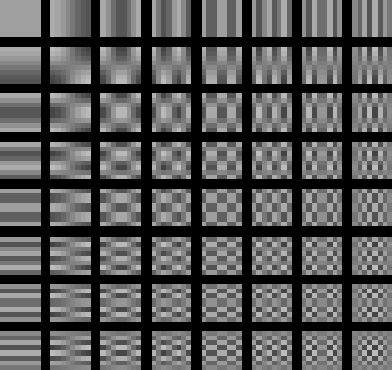
\includegraphics[width=0.6\textwidth]{slike/bazne_funkcije_2D.pdf}
\end{center}
\caption{Dvodimenzionalne bazne funkcije DCT ($N=8$). Srednje siva barva predstavlja ničelno amplitudo, svetlo siva predstavlja pozitivno in temno siva negativno amplitudo. Vir:~\cite{matlab_slika}.}
\label{2D_bazne_funkcije}
\end{figure}

\subsection{Separabilnost} \label{Separabilnost}% vir (https://web.archive.org/web/20150711105353/http://wisnet.seecs.nust.edu.pk/publications/tech_reports/DCT_TR802.pdf)
Eden izmed mnogih razlogov zakaj je DCT postal popularen je dejstvo, da lahko večdimenzionalne verzije DCT izračunamo z zaporednimi enodimenzionalnimi DCT-ji. Pogledali si bomo to na primeru dveh dimenzij. Definicijo dvodimenzionalne DCT \eqref{eq:2D-DCT} lahko zapišemo sledeče
\begin{equation}
    \begin{aligned}
    &C(u,v) = \left(\alpha(u)  \sum_{x=0}^{N-1}\cos\left[\frac{\pi(2x+1)u}{2N}\right]
              \left(\alpha(v)  \sum_{y=0}^{N-1} f(x,y)\cos\left[\frac{\pi(2y+1)u}{2N}\right]\right)\right), \\
    &u,v = 0,1,2,\ldots,N-1.
    \end{aligned}
\label{eq:2D-DCT_Separabilnost}
\end{equation}
Definirajmo še
\begin{equation*}
    g(x) = \left(\alpha(v)  \sum_{y=0}^{N-1} f(x,y)\cos\left[\frac{\pi(2y+1)u}{2N}\right]\right),
\end{equation*}
torej prvo izračunamo $g(x)$ kot da je enodimenzionalen DCT, nato damo ta rezultat v levi del in ponovno izračunamo enodimenzionalen DCT kot $C(u,v) = \alpha(u)  \sum_{x=0}^{N-1}g(x)\cos\left[\frac{\pi(2x+1)u}{2N}\right]$. Pokazali smo torej, da lahko dvodimenzionalni DCT zapišemo kot dva enodimenzionalna DCT-ja.\par
Ta lastnost nam omogoča, da lahko $C(u,v)$ izračunamo v dveh zaporedni enodimenzionalnih operacijah na vrsticah in stolpcih. Ideja je prikazana v Sliki \ref{Prikaz_separabilnosti}. Podobno lahko izpeljemo enačbo \eqref{eq:2D-DCT-inverse} in pokažemo, da je inverzen DCT tudi separabilen.\par


\begin{figure}[ht] % vir (https://web.archive.org/web/20150711105353/http://wisnet.seecs.nust.edu.pk/publications/tech_reports/DCT_TR802.pdf)
\begin{center}
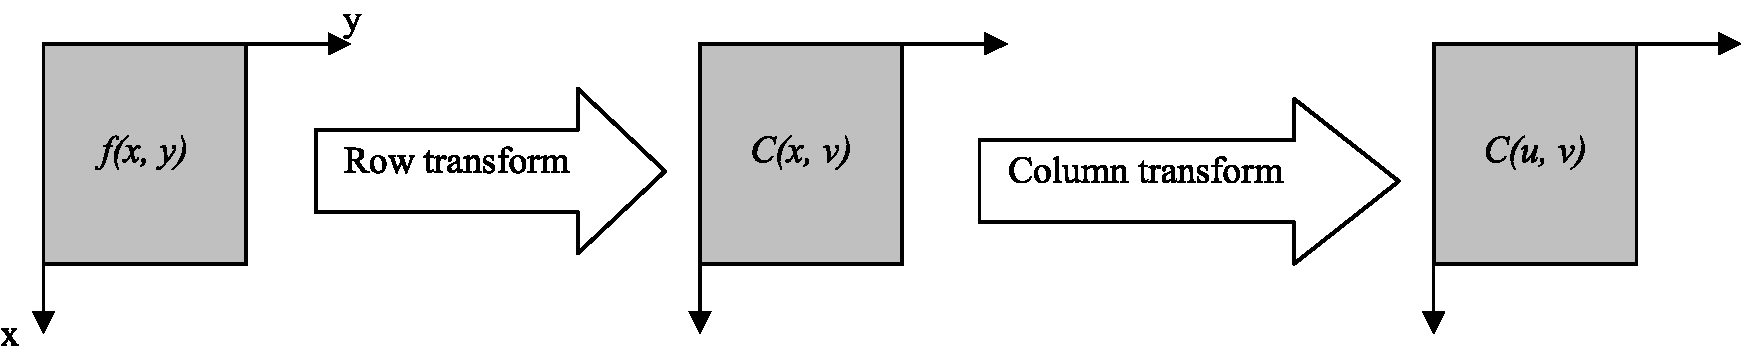
\includegraphics[width=1\textwidth]{slike/Prikaz_Separabilnosti.pdf}
\end{center}
\caption{Dvodimenzionalne bazne funkcije DCT ($N=8$). Srednja siva barva predstavlja ničelno amplitudo, svetlo siva predstavlja pozitivno in temno siva negativno amplitudo. Vir:~\cite{DCT_article}.}
\label{Prikaz_separabilnosti}
\end{figure}

To lastnost bomo potrebovali pri algoritmu za hiter DCT. Ta algoritem bomo pokazali v eni dimenziji in ga nato razširili v dve dimenziji s pomočjo te lastnosti.

\section{Algoritem za hiter DCT}\label{Algoritem za hiter DCT}
V tem razdelku bomo predstavili enega izmed algoritmov za hiter izračun DCT. S tem je mišljen algoritem, kjer je pri $N$ elementih signala časovna zahtevnost $\mathcal{O}(N\log{}N)$. Povzeli bomo algoritem opisan v~\cite{FastDCT}.
Ta algoritem uporablja že obstoječe algoritme za hitro Fourierovo transformacijo (FFT) in njihove rezultate le prilagodi, da ustrezajo definiciji DCT. Obstajajo tudi alternativne izbire, ki ne uporabljajo FFT temveč rekurzivno uporabljajo različne tipe DCT-jev. Primer takšnega algoritma je opisan tudi v~\cite{britanak2010discrete}. Katero implementacijo uporabimo je odvisno kakšne so naše potrebe in zmogljivosti. Odvisno kakšne imamo strojne zmogljivosti so lahko različni algoritmi optimalni. Na primer strojne implementacije direktno na čipih uporabljajo drugačne algoritme kot pa implementaciji v programski opremi na večnamenskih procesorjih. Tukaj predstavljen algoritem je implementiran v programskem jeziku Python, v knjižnici scipy.fftpack pod imenom scipy.fftpack.dct. Tukaj bomo naredili izpeljavo, ki sledi izpeljavi v~\cite{FastDCT}. Ta izpeljava je rahlo prilagojena, saj je v~\cite{FastDCT} uporabljena nestandardna definicija za DCT, kjer je vodilni koeficient drugačen.\par
Želimo izračunati DCT od $f(x)$, ki je zaporedje realnih števil dolžine $N$, torej je definirano na $0 \leq x \leq N-1$. DCT bomo prvo izpeljali iz 2N točkovne diskretne Fourierove transformacije (DFT). Definirajmo 
\begin{equation}
  g(x)=
    \begin{cases}
          f(x), & 0 \leq x \leq N-1 \\
          f(2N-x-1), & N \leq x \leq 2N-1 \\
    \end{cases}.
\label{eq:fastDCT_y}
\end{equation}

Velja $g(2N-x-1) = g(x)$.
Definirajmo DFT od $g(x)$ kot
\begin{equation}
  G(u) = \sum_{x=0}^{2N-1} g(x) W_{2N}^{xu},
\label{eq:DFT}
\end{equation}
kjer je $W_{2N}$ $2N$-ti koren enote, torej
\begin{equation}
  W_{2N} = e^{-i2\pi/2N}.
\label{eq:DFT_W}
\end{equation}

Če zamenjamo \eqref{eq:fastDCT_y} v \eqref{eq:DFT} dobimo
\begin{equation}
  G(u) = \sum_{x=0}^{N-1} f(x) W_{2N}^{xu} + \sum_{x=N}^{2N-1} x(2N-x-1) W_{2N}^{xu}.
\label{eq:DFT_z_g1}
\end{equation}
V desni vsoti uporabimo novo spremenljivko vsote in upoštevamo, da je $W_{2N}^{2mN} = 1$ za $\forall m \in \mathbb{Z}$. Izpostavimo $W_{2N}^{-u/2}$ in dobimo
\begin{equation}
  G(u) = W_{2N}^{-u/2}\sum_{x=0}^{N-1} f(x) \left[ W_{2N}^{xu}W_{2N}^{u/2} + W_{2N}^{-xu}W_{2N}^{-u/2} \right].
\label{eq:DFT_z_g2}
\end{equation}
Izraz v \eqref{eq:DFT_z_g2} lahko zapišemo na dva načina
\begin{equation}
  G(u) = W_{2N}^{-u/2} 2 \sum_{x=0}^{N-1} f(x) \cos\frac{\pi(2x+1)u}{2N}, \indent 0 \leq u \leq 2N-1
\label{eq:DFT_z_enacbo_DCT}
\end{equation}

ali

\begin{equation}
  G(u) = W_{2N}^{-u/2} 2 \mbox{Re} \left[ W_{2N}^{u/2} \sum_{x=0}^{N-1} f(x) W_{2N}^{xu} \right], \indent 0 \leq u \leq 2N-1
\label{eq:DFT_z_Re},
\end{equation}
kjer oznaka Re pomeni, da vzamemo realno komponento kompleksnega šte\-vi\-la.
Vstavimo definicijo DCT iz \eqref{eq:1D-DCT} v \eqref{eq:DFT_z_enacbo_DCT} in dobimo

\begin{equation}
  G(u) = W_{2N}^{-u/2} \frac{2}{\alpha(u)} C(u)
\label{eq:DFT_z_DCT}
\end{equation}
ali
\begin{equation}
  C(u) = W_{2N}^{u/2} \frac{\alpha(u)}{2} G(u).
\label{eq:DCT_z_DFT}
\end{equation}
Vstavimo \eqref{eq:DFT_z_Re} v \eqref{eq:DCT_z_DFT} dobimo

\begin{equation}
  G(u) = \alpha(u)\mbox{Re}\left[ W_{2N}^{u/2} \sum_{x=0}^{N-1} f(x) W_{2N}^{xu} \right], \indent 0 \leq u \leq 2N-1.
\label{eq:DCT_z_Re}
\end{equation}
Za izračun DCT torej uporabimo 2N točkovni FFT od $g(x)$, njegove rezultate nato vstavimo v \eqref{eq:DCT_z_DFT} in dobimo DCT. V \eqref{eq:DCT_z_Re} vidimo, da lahko DCT od $f(x)$ dobimo tudi tako, da izračunamo 2N točkovni DFT originalnega $f(x)$ z $N$ ničlami dodanimi na koncu. Nato pomnožimo rezultat s $W_{2N}^{u/2}$, vzamemo realni del tega in pomnožimo z $\alpha(u)$.\par
Ta algoritem velja za hitrega saj bomo za izračun DFT v \eqref{eq:DCT_z_DFT} uporabili FFT, ki se za zaporedje dolžine $n$ izračuna v $\mathcal{O}(n\log{}n)$ korakih. Več informacij o tem zakaj je FFT tako hiter in njegova psevdokoda je na voljo v \cite{Kozak_1997}. Tukaj smo imeli DFT na $2N$ točkah, kar nam da časovno zahtevnost $\mathcal{O}(2N\log{}2N)$, kar je enako $\mathcal{O}(N\log{}N)$. Potrebujemo še pri vsakem koeficientu nekaj množenj, deljenj in izračun $W_{2N}^{-u/2}$, kar skupaj za vse koeficiente naredimo v $\mathcal{O}(n)$ korakih. Skupna časovna zahtevnost hitrega DCT je torej $\mathcal{O}(N\log{}N)$ za signal dolžine $N$. Z uporabo tega algoritma smo torej prišli iz časovne zahtevnosti $\mathcal{O}(N^2)$ na $\mathcal{O}(N\log{}N)$. To je velika izboljšava.



Sedaj potrebujemo še hiter inverzni DCT. Tega izpeljemo na podoben način, kjer prvo vzamemo inverzni DFT. Inverzni DFT od $G(u)$ je definiran kot 
\begin{equation}
  G(u) = \frac{1}{2N}\sum_{u=0}^{2N-1} G(u) W_{2N}^{-xu}.
\label{eq:Inverse_DFT}
\end{equation}
Ker je $g(x)$ realna funkcija je posledično njen DFT $G(x)$ Hermitsko simetričen, torej
\begin{equation}
  G(2N - u) = G\text{*}(u).
\label{eq:Hermitska_simetricnost}
\end{equation}
Potrebujemo tudi, da po \eqref{eq:DFT_z_Re} velja
\begin{equation}
  G(N) = 0.
\label{eq:G(N)=0}
\end{equation}
Če vstavimo \eqref{eq:Hermitska_simetricnost} in \eqref{eq:G(N)=0} v \eqref{eq:Inverse_DFT} dobimo 
\begin{equation}
  g(x) = \frac{1}{N}\mbox{Re}\left[ \frac{G(0)}{2} + \sum_{u=1}^{N-1} G(u) W_{2N}^{-xu}   \right], \indent 0 \leq x \leq 2N-1.
\label{eq:Inverse_DCT_z_DFT}
\end{equation}
Če vstavimo \eqref{eq:DFT_z_DCT} v \eqref{eq:Inverse_DCT_z_DFT} in uporabimo \eqref{eq:fastDCT_y} dobimo inverzni DCT kot zapisan v \eqref{eq:1D-DCT-inverse}.\par
Torej če imamo dan $C(u)$ dobimo $f(x)$ tako, da prvo izračunamo $G(u)$ po \eqref{eq:DFT_z_DCT}. Nato s pomočjo \eqref{eq:Inverse_DCT_z_DFT} dobimo $g(x)$ in iz njega pridobimo $f(x)$ po \eqref{eq:fastDCT_y}.\par
Ta algoritem ima tudi časovno zahtevnost $\mathcal{O}(N\log{}N)$, ker deluje zelo podobno kot DCT. Najprej ima nekaj množenj, deljenj in izračun $W_{2N}^{-u/2}$ isto kot DCT. Nato pa uporabimo inverzen FFT, ki ima časovno zahtevnost $\mathcal{O}(N\log{}N)$.\par
Pomembno je omeniti tudi, da obstaja je ta algoritem za izračun DCT, numerično stabilen. Brez te lastnosti bi bila ta metoda popolnoma neuporabna.





\begin{comment}
V~\cite{FastDCT} je izpeljano, da lahko zapišemo DCT od $f(x)$ kot
\begin{equation}
  C(u) = \alpha(u)\mbox{Re}\left[ W_{4N}^{u} \sum_{x=0}^{N-1} v(x) W_N^{xu}\right], \indent 0 \leq u \leq N-1
\label{eq:DCT_z_DFT_Dolzine_N}
\end{equation}
Tukaj vidimo da je $\sum_{x=0}^{N-1} v(u) W_N^{xu}$ DFT od $v(u)$ z $N$ točkami, kar se bo izračunalo s hitrim algoritmom za DFT, ki se mu reče FFT. Kasneje bomo zapisali psevdokodo algoritma FFT.\par

Sedaj izračunajmo še inverzni DCT s pomočjo inverznega DFT.

\begin{equation}
  v(u) = \frac{1}{N} \sum_{x=0}^{N-1} V(u) W_{N}^{-xu}
\label{eq:inverse_DFT}
\end{equation}

Po izpeljavi v~\cite{FastDCT} je najprej potrebno izračunati $V(u)$ kot


\begin{equation}
  V(u) = \frac{1}{2} W_{4N}^{-u}\left[ C(u) - iC(N-u) \right], \indent 0 \leq u \leq N-1
\label{eq:izracun_V}
\end{equation}
V tej definiciji 

% potrebno pokazat, da lahko izračunamo DCT z (N/2) kompleksnim IDFT. To se naredi tako, da se uporabi hermetsko simetrično zaporedja.(zapisano v Appendix od članka)!!!!!!!!!!!!!!!!!!!!


    

\begin{equation}
  v(x)=
    \begin{cases}
          f(2x), & 0 \leq x \leq \lfloor\frac{N-1}{2}\rfloor \\
          f(2N-2x-1), & \lfloor\frac{N+1}{2}\rfloor \leq x \leq N-1 \\
    \end{cases}.
\label{eq:fastDCT_v}
\end{equation}
Ta definicija pravi, da najprej vzamemo sode točke $f(x)$ po vrsti in za njimi lihe točke v obratnem vrstnem redu.
\end{comment}


\section{Integer DCT}
Pokazali bomo eno metodo aproksimacije DCT s celimi števili. To je zaželeno zaradi bolj enostavne aritmetike pri računanju s celimi števili. Implementacijo, ki si bomo ogledali tukaj je z množenjem in seštevanje celih števil. Obstajajo sicer tudi implementacije, ki uporabljajo zgolj binarno seštevanje in operacijo bitnega premika (\textit{angl.} bit shift). Tukaj se lahko običajno dosežejo boljši rezultati v primeru, da uporabljamo števila z več biti. Posledično se sicer poveča računska zahtevnosti. Predstavili bomo eno izmed bolj enostavnih implementacij celo\-šte\-vil\-ske\-ga DCT, ki je opisana v~\cite{britanak2010discrete}. Ista knjiga vsebuje tudi bolj napredne implementacije v katere se tukaj ne bomo poglabljali.\par
Pokazali bomo korake kako pretvoriti realno številski DCT v celoštevilski DCT. Tukaj si bomo ogledali samo primer, ko je $N=8$, zaradi enostavnosti razlage. V splošnem je ta primer tudi najbolj pogosto uporabljan. Torej želimo aproksimirati DCT matriko $C_8$, ki smo jo definirali v \eqref{eq:1D_DCT_matrika}, z $\widetilde{C_8}$. $\widetilde{C_8}$ bo definirana kot
\begin{equation}
  \widetilde{C_8} = Q_8 V_8.
\label{eq:c_8}
\end{equation}
V tem zapisu $Q_8$ predstavlja diagonalno matriko z normalizacijskimi faktorji na glavni diagonali. Ti niso nujno celoštevilski, potrebujemo jih, da bo naša DCT ortogonalna. 

\begin{comment}
Postopek pridobitve $\widetilde{C_8}$ iz $C_8$ je sledeč. Najprej bomo generirali $C_8$ v ekspicitni in numerični obliki

\begin{gather*}
 C_8 = \frac{1}{2}
  \setlength{\arraycolsep}{1pt}
  \renewcommand{\arraystretch}{1}
  \begin{bmatrix}
  \frac{1}{\sqrt{2}} & \frac{1}{\sqrt{2}} & \frac{1}{\sqrt{2}} & \frac{1}{\sqrt{2}} & \frac{1}{\sqrt{2}} & \frac{1}{\sqrt{2}} & \frac{1}{\sqrt{2}} & \frac{1}{\sqrt{2}}\\
  \cos{\frac{\pi}{16}} & \cos{\frac{3\pi}{16}} & \sin{\frac{3\pi}{16}} & \sin{\frac{\pi}{16}} & -\sin{\frac{\pi}{16}} & -\sin{\frac{3\pi}{16}} & -\cos{\frac{3\pi}{16}} & -\cos{\frac{\pi}{16}}\\
  \cos{\frac{\pi}{8}} & \sin{\frac{\pi}{8}} & -\sin{\frac{\pi}{8}} & -\cos{\frac{\pi}{8}} & -\cos{\frac{\pi}{8}} & -\sin{\frac{\pi}{8}} & \sin{\frac{\pi}{8}} & \cos{\frac{\pi}{8}} \\
  \cos{\frac{3\pi}{16}} & -\sin{\frac{\pi}{16}} & -\cos{\frac{\pi}{16}} & -\sin{\frac{3\pi}{16}} & \sin{\frac{3\pi}{16}} & \cos{\frac{\pi}{16}} & \sin{\frac{\pi}{16}} & -\cos{\frac{3\pi}{16}}\\
  \frac{1}{\sqrt{2}} & -\frac{1}{\sqrt{2}} & -\frac{1}{\sqrt{2}} & \frac{1}{\sqrt{2}} & \frac{1}{\sqrt{2}} & -\frac{1}{\sqrt{2}} & -\frac{1}{\sqrt{2}} & \frac{1}{\sqrt{2}}\\
  \sin{\frac{3\pi}{16}} & -\cos{\frac{\pi}{16}} & \sin{\frac{\pi}{16}} & \cos{\frac{3\pi}{16}} & -\cos{\frac{3\pi}{16}} & -\sin{\frac{\pi}{16}} & \cos{\frac{\pi}{16}} & -\sin{\frac{3\pi}{16}}\\
  \sin{\frac{\pi}{8}} & -\cos{\frac{\pi}{8}} & \cos{\frac{\pi}{8}} & -\sin{\frac{\pi}{8}} & -\sin{\frac{\pi}{8}} & \cos{\frac{\pi}{8}} & -\cos{\frac{\pi}{8}} & \sin{\frac{\pi}{8}} \\
  \sin{\frac{\pi}{16}} & -\sin{\frac{3\pi}{16}} & \cos{\frac{3\pi}{16}} & -\cos{\frac{\pi}{16}} & \cos{\frac{\pi}{16}} & -\cos{\frac{3\pi}{16}} & \sin{\frac{3\pi}{16}} & -\sin{\frac{\pi}{16}}\\
   \end{bmatrix}
\end{gather*}
Označimo s $c_{ij}$ koeficiente tabele $C_8$. Če gledamo absolutne vrednosti elementov $C_8$ vidimo sledeče
\begin{alignat*}{1}
    & |c_{00}| = |c_{01}| = |c_{02}| = |c_{03}| = |c_{04}| = |c_{05}| = |c_{06}| = |c_{07}| = \\
    &  = |c_{40}| = |c_{41}| = |c_{42}| = |c_{43}| = |c_{44}| = |c_{45}| = |c_{46}| = |c_{47}| = \frac{1}{\sqrt{2}},\\
    & |c_{10}| = |c_{17}| = |c_{32}| = |c_{35}| = |c_{51}| = |c_{56}| = |c_{73}| = |c_{74}| = \cos{\frac{\pi}{16}},\\
    & |c_{11}| = |c_{16}| = |c_{30}| = |c_{37}| = |c_{53}| = |c_{54}| = |c_{72}| = |c_{75}| = \cos{\frac{3\pi}{16}},\\
    & |c_{12}| = |c_{15}| = |c_{33}| = |c_{34}| = |c_{50}| = |c_{57}| = |c_{71}| = |c_{76}| = \sin{\frac{3\pi}{16}},\\
    & |c_{13}| = |c_{14}| = |c_{31}| = |c_{36}| = |c_{52}| = |c_{55}| = |c_{70}| = |c_{77}| = \sin{\frac{\pi}{16}},\\
    & |c_{20}| = |c_{23}| = |c_{24}| = |c_{27}| = |c_{61}| = |c_{62}| = |c_{65}| = |c_{66}| = \cos{\frac{\pi}{8}},\\
    & |c_{21}| = |c_{22}| = |c_{25}| = |c_{26}| = |c_{60}| = |c_{63}| = |c_{64}| = |c_{67}| = \sin{\frac{\pi}{8}}.
\end{alignat*}
\end{comment}
V eksplicitnem zapisu $C_8$ opazimo, da ima le 7 različnih vrednosti. Zapišemo elemente z enako magnitudo z isto spremenljivko iz množice $\{a,b,c,d,e,f,g\}$, kjer so $a,b,c,d,e,f,g \in \mathbb{N}$. Definirajmo $V_8$ tako, da ohranimo istoležne predznake od $C_8$ in na mestih, kjer ima $C_8$ števila enake magnitude dajmo isto spremenljivko. Izrazimo $\widetilde{C_8}$ po tej definiciji
\begin{gather}
   \widetilde{C_8} = Q_8
 \begin{bmatrix}
    g&  a&  e&  b&  g&  c&  f&  d\\
    g&  b&  f& -d& -g& -a& -e& -c\\
    g&  c& -f& -a& -g&  d&  e&  b\\
    g&  d& -e& -c&  g&  b& -f& -a\\
    g& -d& -e&  c&  g& -b& -f&  a\\
    g& -c& -f&  a& -g& -d&  e& -b\\
    g& -b&  f&  d& -g&  a& -e&  c\\
    g& -a&  e& -b&  g& -c&  f& -d\\
 \end{bmatrix}.
\label{eq:IntegerDCT_Q8}
\end{gather}
Želimo, da sta i-ti in j-ti bazni vektor ortogonalna. Označimo i-ti in j-ti stolpec $V_8$ kot $v^{(i)} $ in $v^{(j)}$. Ta vektorja sta ortogonalna, če je njun skalarni produkt 0 torej
\begin{equation*}
    (v^{(i)}) (v^{(j)})^T = \sum_{k=0}^7v^{(i)}_{k}v^{(j)}_{k} = 0,\indent \forall i \neq j, \indent i,j = 0,1,\ldots,7.
\end{equation*}

Za ortogonalnost matrike potrebujemo še, da je norma stolpcev $\widetilde{C_8}$ enaka 1. Najprej definirajmo drugo normo baznega vektorja
\begin{equation}
    \lVert v^{(i)} \rVert_2 = \sqrt{\sum_{k=0}^7 (v^{(i)}_{k})^2}, \indent i,k = 0,1,\ldots,7.
\end{equation}
Definirajmo še 
\begin{equation}
    q_{ii} = \lVert v^{(i)} \rVert_2^2.
\end{equation}
Sedaj lahko definiramo matriko $Q_8$ kot
\begin{equation}
    Q_8 = \hbox{diag}\left(\frac{1}{\sqrt{q_{00}}},\ldots,\frac{1}{\sqrt{q_{77}}}\right).
\end{equation}
Ta definicija zagotovi, da bo $\widetilde{C_8}$ ortogonalna. Členi $\frac{1}{\sqrt{q_{ii}}}$ so v splošnem iracionalna števila. Temu se ne moramo izogniti, če želimo imeti ortogonalni DCT. Pogoj za ortogonalnost lahko zapišemo tudi kot
\begin{equation}
    V_8 V_8^T = [Q_8^{-1}]^2I_8.
\end{equation}
Iz tega pogoja pridobimo enačbo
\begin{equation}
    a(b-c)-d(b+c) = 0
\label{eq:integerDCT_pogoj}
\end{equation}
in
\begin{equation}
  \begin{aligned}
    &q_{00} = q_{44} = 8g^2,\\
    &q_{11} = q_{33} = q_{55} = q_{77} = 2(a^2 + b^2 + c^2 + d^2),\\
    &q_{22} = q_{66} = 4(e^2 + f^2).
  \end{aligned}
\label{eq:integerDCT_q_ii}
\end{equation}
Iz teh pogojev vidimo, da lahko spremenljivke $e$, $f$ in $g$ obravnavamo ločeno od $a$, $b$, $c$ in $d$.\par
Določiti moramo še nekaj neenakosti med temi koeficienti, da bodo magnitude baznih vektorjev $V_8$ približno enako tistim v matriki $C_8$. Z upo\-šte\-van\-jem \eqref{eq:integerDCT_pogoj} in \eqref{eq:integerDCT_q_ii} lahko določimo sledeče neenakosti
\begin{align} 
  \label{eq:integerDCT_neenakost_1}
  &a > b > c > d > 0, \\
  \label{eq:integerDCT_neenakost_2}
  &a > e > f > 0, \\
  \label{eq:integerDCT_neenakost_3}
  &a > g > 0.
\end{align}
Želimo najti množico celih števil $\{a,b,c,d,e,f,g\}$, ki zadoščajo enakosti \eqref{eq:integerDCT_pogoj} in neenakostim \eqref{eq:integerDCT_neenakost_1}-\eqref{eq:integerDCT_neenakost_3}. Za rešitev te enačbe lahko iščemo števila v množici $\{a,b,c,d,e,f,g\}$, ki so predstavljena z $M$ biti. V splošnem je tukaj lahko neskončno rešitev enačbe s temi omejitvami. DCT s celimi števili je določena s $\{a,b,c,d,e,f,g\}$, kar bomo označili kot $IntegerDCT_8(a,b,c,d,e,f,g)$. Izbrano množico $\{a,b,c,d,e,f,g\}$ bomo vstavili v matriko $V_8$ kot definirano v \eqref{eq:IntegerDCT_Q8}. Podobno vstavimo vse $q_{ii}$ dane v \eqref{eq:integerDCT_q_ii} vstavimo v $Q_8$. Vse rešitve, ki upoštevajo enačbo \eqref{eq:integerDCT_pogoj} in omejitve \eqref{eq:integerDCT_neenakost_1}-\eqref{eq:integerDCT_neenakost_3} nam bodo dalo matriko $\widetilde{C_8}$, ki je ortogonalna in blizu matriki $C_8$. Efektivnost implementacije $IntegerDCT_8(a,b,c,d,e,f,g)$ bo odvisna predvsem od izbire velikosti koeficientov, torej kako velik $M$ bomo dovolili.\par
Tukaj bomo povedali nekaj primerov, ko bodo $e=3$, $g=1$ in $f =1$. To je izbira opisana v~\cite{britanak2010discrete}. Torej pogledali si bomo nekaj primerov $IntegerDCT_8(a,b,c,d,3,1,1)$, kjer bomo za M vzeli vrednosti 3, 4, 5, 6, 7 ali 8. Za mero točnosti specifičnega približka bomo pa uporabili mero srednje kvadratne napake, ki jo označimo z MSE (\textit{angl.} Mean squared error) in je definirana kot
\begin{equation} % moram nekje najdit da bom citiral tako verzijo definicije
  \hbox{MSE}(X, \widetilde{X}) = \frac{1}{mn}\sum_{i=0}^{i=n-1}\sum_{j=0}^{j=m-1}\left(X_{ij} - \widetilde{X_{ij}} \right)^2.
\label{eq:MSE}
\end{equation}
Tukaj je $X$ originalna matrika in $\widetilde{X}$ približek originalni matriki.\par
Primerjali bomo MSE različnih $IntegerDCT_8(a,b,c,d,3,1,1)$ v primerjavi z originalnim DCT v Tabeli \ref{tab:IntegerDCT_8}

\begin{table}[ht]
\centering
\begin{tabular}{|l|c|}
\hline
$IntegerDCT_8(a,b,c,d,3,1,1)$              &MSE          \\
\hline
$DCT                                     $ &0             \\
$IntegerDCT_8(5, 3, 2, 1, 3, 1, 1)       $ &2.721681e-003\\ 
$IntegerDCT_8(10, 9, 6, 2, 3, 1, 1)      $ &2.060647e-004\\ 
$IntegerDCT_8(15, 12, 8, 3, 3, 1, 1)     $ &2.059246e-004\\ 
$IntegerDCT_8(25, 21, 14, 5, 3, 1, 1)    $ &1.302862e-004\\ 
$IntegerDCT_8(45, 39, 26, 9, 3, 1, 1)    $ &1.380974e-004\\ 
$IntegerDCT_8(55, 48, 32, 11, 3, 1, 1)   $ &1.458331e-004\\ 
$IntegerDCT_8(65, 57, 38, 13, 3, 1, 1)   $ &1.524257e-004\\ 
$IntegerDCT_8(120, 105, 70, 24, 3, 1, 1) $ &1.492797e-004\\ 
$IntegerDCT_8(175, 153, 102, 35, 3, 1, 1)$ &1.481648e-004\\ 
$IntegerDCT_8(230, 201, 134, 46, 3, 1, 1)$ &1.475946e-004\\ 
\hline
\end{tabular}
\caption{Tabela različnih možnih $IntegerDCT_8(a,b,c,d,3,1,1)$ s pripadajočimi MSE od originalnega DCT}
\label{tab:IntegerDCT_8}
\end{table}
Izpišimo še en primer tabele $\widetilde{C_8}$ za primer $IntegerDCT_8(15, 12, 8, 3, 3, 1, 1)$

\begin{gather}
   \widetilde{C_8} = Q_8
 \begin{bmatrix} 
    1& 15&  3& 12&  1&  8&  1&  3\\ 
    1& 12&  1& -3& -1&-15& -3& -8\\
    1&  8& -1&-15& -1&  3&  3& 12\\
    1&  3& -3& -8&  1& 12& -1&-15\\
    1& -3& -3&  8&  1&-12& -1& 15\\
    1& -8& -1& 15& -1& -3&  3&-12\\
    1&-12&  1&  3& -1& 15& -3&  8\\ 
    1&-15&  3&-12&  1& -8&  1& -3\\
 \end{bmatrix}
\label{eq:IntegerDCT_8(15, 12, 8, 3, 3, 1, 1)}
\end{gather}


kjer so $q_{ii}$ dani kot
\begin{equation}
  \begin{aligned}
    &q_{00} = q_{44} = 1,\\
    &q_{11} = q_{33} = q_{55} = q_{77} = 884,\\
    &q_{22} = q_{66} = 10,
  \end{aligned}
\end{equation}
torej je
\begin{equation}
    Q_8 = \hbox{diag}\left(\frac{1}{\sqrt{8}}, \frac{1}{\sqrt{442}},\frac{1}{\sqrt{40}},\frac{1}{\sqrt{442}},\frac{1}{\sqrt{8}},\frac{1}{\sqrt{442}},\frac{1}{\sqrt{40}},\frac{1}{\sqrt{442}}, \right).
\end{equation}
Tukaj smo zapisali samo matriko s katero bi morali množiti vektor vrednosti signala, da bi dobili DCT. V knjigi~\cite{britanak2010discrete} so zapisane še izboljšave tega algoritma in opisan je tudi način kako lahko tak DCT izračunamo v podobnem številu korakov kot smo pokazali pri hitri verziji navadnega DCT.






\chapter{JPEG}
\label{JPEG}
Format JPEG je izdan v standardu ISO/IEC 10918. Ime dobi od skupine, ki ga je ustvarila, ki se imenuje Joint Photographic Experts Group. Izdan je bil leta 1992 z~\cite{ISO/IEC_10918-1}.\par
JPEG standard določa zgolj ogrodje formata, ki poda nekatere zahteve in predloge za uporabo. Ponuja veliko število opcijskih implementacij, ki so odvisne od namenjene uporabe in od potrebe po moči kompresije. Tukaj bomo predstavili podrobneje zgolj eno izmed bolj popularnih izvedb uporabe tega formata. Opis delovanja JPEG-a je povzet po~\cite{ISO/IEC_10918-1, wallace1992jpeg}.\par 

JPEG podpira štiri različne načine delovanja. Prve trije od teh uporabljajo kompresijo z izgubo in zadnja uporablja kompresijo brez izgub.
\begin{itemize}
   \item Zaporedno kodiranje (\textit{angl.} Sequential encoding): slika je kodirana od leve proti desni in od vrha do dna.
   \item Progresivno kodiranje (\textit{angl.} Progressive encoding): slika je kodirana v več obhodih za aplikacije, kjer je čas prenosa dolg. Tukaj ob dekodiranju takoj dobimo nizko resolucijo slike, ki z obhodi pridobiva na ločljivosti.
   \item Hierarhično kodiranje (\textit{angl.} Hierarchical encoding): slika je kodirana pri več različnih resolucijah. Na ta način lahko dostopamo do nižjih resolucij brez da bi morali dekompresirati slika pri polni resoluciji.
   \item Kodiranje brez izgub (\textit{angl.} Lossless encoding): slika je kodirana, da ob dekodiranju dobimo identično kopijo originala (ta način delovanja, da zelo minimalno kompresijo)
\end{itemize}
Vsak od teh načinov delovanja ima kasneje še specificiranih več različnih kodekov (par kodirnika in dekodirnika).
Od sedaj naprej bomo govorili zgolj o zaporednem kodiranju, saj je to najpogostejša implementacija v današnjih programih.\par
Na sliki \ref{Shema_JPEG} je prikazana osnovna shema kodiranja slike v JPEG formatu.
\begin{figure}[ht] % vir (https://www.w3.org/Graphics/JPEG/itu-t81.pdf)
\begin{center}
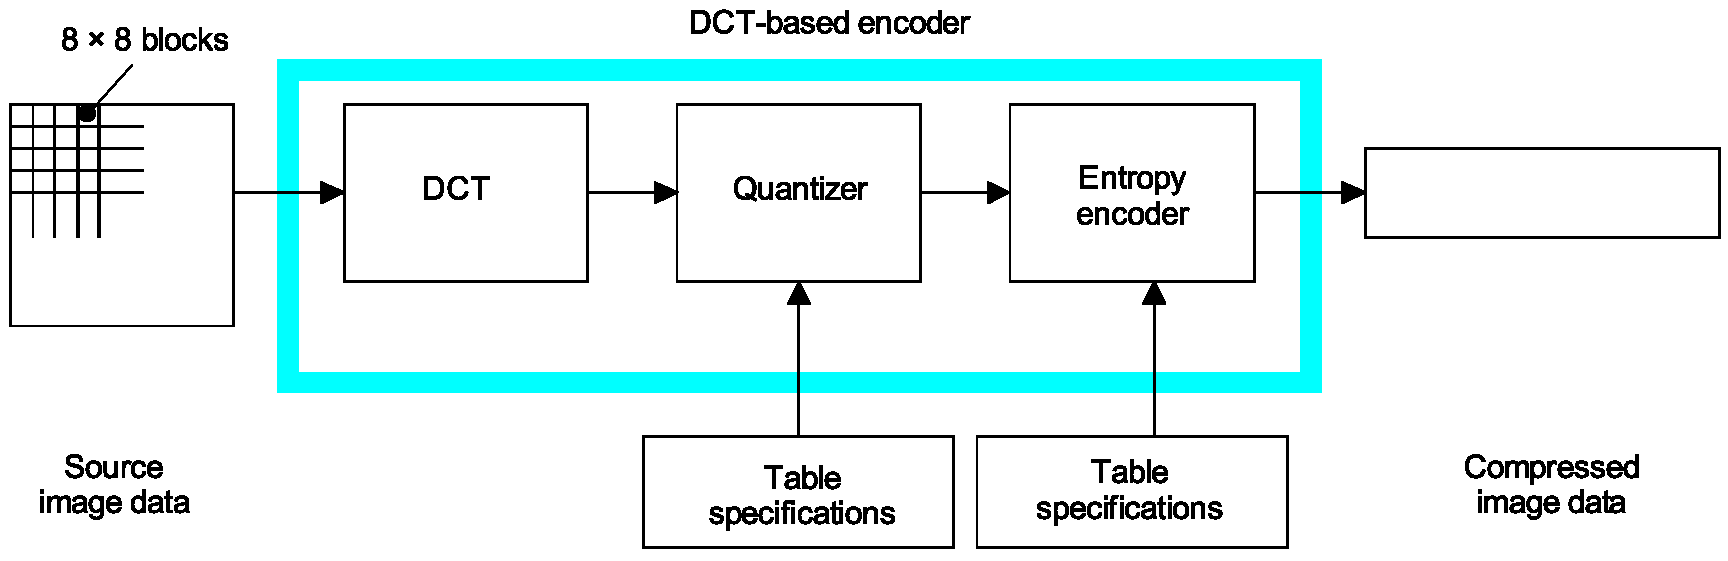
\includegraphics[width=0.9\textwidth]{slike/Shema_JPEG.pdf}
\end{center}
\caption{Shema kodiranja JPEG-a. Vir:~\cite{ISO/IEC_10918-1}.}
\label{Shema_JPEG}
\end{figure}
Predstavili bomo vse procese potrebne, da bomo znali preslikati sliko v končno bitno zaporedje, ki se shrani in pošilja med napravami. V prvem delu bomo o tem kako se obravnavajo barvni kanali. Za to se uporablja barvno podvzorčenje (\textit{angl.} chroma subsampling). O njem ne bomo šli v podrobnosti, saj so za nas zgolj pomembni prihranki. Več informacij o barvnem podvzorčenju je na voljo v~\cite{chroma_subsampling}. Od tu dalje bomo delali na 8x8 blokih slike, kot je prikazano na Sliki \ref{Shema_JPEG}. Na teh blokih bomo izvedli DCT, ki ga nato kvantiziramo (\textit{angl.} quantization), torej odstranijo se manj pomembni podatki. Pokazali bomo kako se ti podatki nato pripravijo za kodiranje. Na teh podatkih se izvede entropijsko kodiranje (\textit{angl.} entropy encoding) s Huffmanovim kodiranjem. O njem ponovno ne bomo veliko povedali, saj bomo pokazali primer, kjer imamo podano tabelo za Huffmanovo kodiranje. Torej bomo samo uporabili tabelo za povprečno sliko in ne bomo izgrajevali svojih. Več informacij o Huffmanovem kodiranju je na voljo v~\cite{huffman_coding}. Na koncu bomo dobili niz bitov, ki predstavlja blok slike.

\section{Predprocesiranje}
Osnovni format JPEG sam po sebi ne določi veliko o barvnih kanalih. Lahko ga uporabljamo za slike v sivinah (\textit{angl.} grayscale images), kar je najbolj enostaven primer, saj tu imamo zgolj en barvni kanal. V tem primeru se ta barvni kanal lahko direktno pošlje dalje. Bolj pogosto se uporabljajo barvne slike. Te imajo običajno tri barvne kanale. Najpogostejši od teh zapisov je v oblike RGB, kjer imamo po en kanal za rdečo, zeleno in modro intenziteto. Te bi lahko obravnavali kot neodvisne in jih ločeno poslali dalje ter jih šele ob dekodiranju nazaj združili. Bolj uspešen način za višjo kompresijo je, da jih preslikamo v barvni prostor, kjer se loči svetilnost (\textit{angl.} luminance) in barvo (\textit{angl.} chrominance). Torej bomo iz RGB prostora preslikali v prostor Y'C\textsubscript{B}C\textsubscript{R}, kjer Y' predstavlja svetilnost, medtem ko C\textsubscript{B} in C\textsubscript{R} predstavljata barvo. To naredimo, ker je človeško oko bolj občutljivo na svetilnost kot na barvo. Nato bomo izvedli barvno podvzorčenje preden pošljemo sliko dalje. Najpogosteje se uporablja barvno podvzorčenje 4:2:2 ali 4:2:0. Prvi iz barvnih kanalov odstrani $1/2$ podatkov torej, če gledamo celotne podatke tu odstranimo $1/3$. V drugem primeru odstranimo $3/4$ barvnih podatkov, torej v celoti $1/2$ podatkov. Tu se zmanjša resolucija drugih dveh kanalov, ko jih pošljemo dalje. \par
% vir za chroma subsampling https://www.researchgate.net/publication/321286841_Chroma_Subsampling_Influence_on_the_Perceived_Video_Quality_for_Compressed_Sequences_in_High_Resolutions

Preden razdelimo sliko na bloke je potrebno dodat dovolj pikslov, da bo število pikslov v vodoravni in navpični smeri deljivo z 8. Kako se to naredi ni specificirano v standardu. Ena od pogostejših metod je, da zrcalimo najbolj robne piksle (\textit{angl.} Reflection padding). Nato razdelimo sliko na bloke velikosti 8x8. Označimo vrednosti v teh blokih z $f(x,y)$, kjer je $x,y = 0,1,2,\ldots,7$. Izbira velikosti bloka je 8x8, zaradi hitre izračunljivosti in hkrati dobimo zelo dobre rezultate pri kompresiji in vizualni ločljivosti slik. V teh blokih nato vrednosti zamaknemo iz nepredznačenih celih števil na intervalu $\left[0,2^P-1\right]$ v predznačena cela števila na interval$\left[-2^{P-1},2^{P-1}-1\right]$. Tukaj $P$ označuje število bitov, ki predstavljajo intenziteto piksla v tem barvnem kanalu. Običajno je $P=8$. To pomeni, če označimo z $z$ vrednost piksla, izračunamo nov $z'$ kot $z' = z - 2^{P-1}$

\section{Kodiranje}

Sedaj gre tak 8x8 blok skozi DCT, torej uporabi se formula \eqref{eq:2D-DCT}, kjer je $N=8$. Poenostavljeno zapisano sledeče
\begin{equation}
    \begin{aligned}
    &C(u,v) = \alpha(u) \alpha(v) \sum_{x=0}^{7}\sum_{y=0}^{7} f(x,y)
    \cos\left[\frac{\pi(2x+1)u}{16}\right]
    \cos\left[\frac{\pi(2y+1)u}{16}\right], \\
    &u,v = 0,1,2,\ldots,7.
    \end{aligned}
\label{eq:2D-DCT_JPEG}
\end{equation}
\begin{equation}
\alpha(u)=
    \begin{cases}
          \sqrt{\frac{1}{8}} & \text{za $u=0$} \\
          \sqrt{\frac{1}{4}} & \text{za $u\neq 0$} \\
    \end{cases}.
\label{eq:definicija_alpha_JPEG}
\end{equation}
V praksi se uporabijo hitrejše metode za izračun DCT kot na primer algoritem, ki smo ga predstavili v poglavju \ref{Algoritem za hiter DCT}. V formatu JPEG ni predpisan specifičen način izračuna DCT, saj so pri različnih aplikacij različne implementacije optimalne. Različne implementacije sicer lahko privedejo do različnih rezultatov. Iz tega razloga zahtevajo le, da je algoritem znotraj mer njihovega testa natančnosti. \par

Drugi večji korak je kvantizacija izhoda DCT. Kvantizacija tukaj pomeni, da zmanjšano vpliv manj pomembnih koeficientov, torej te koeficiente delimo z večjimi števili. Tukaj so vsi elementi kvantizirani s pomočjo kvantizacijske tabele velike 8x8, ki je specificirana od uporabnika ali aplikacije. Elemente te tabele označimo s $Q(u,v)$. To so cela števila med 1 in 255, ki določijo koliko se kvantizira pripadajoč DCT koeficient. Kvantizirani koeficienti so izračunani s pomočjo naslednje formule
\begin{equation}
C^Q(u,v) = \hbox{Integer round} \left(\frac{C(u,v)}{Q(u,v)} \right).
\label{eq:kvantizacija}
\end{equation}
To storimo za vse $u,v = 0,\ldots,7$.\par
Ta korak je glavni vir izgube znotraj JPEG-a. Iz tega razloga je kompresija končne slike odvisna predvsem od izbire kvantizacijskih tabel. Primer takšnih tabel je podan v~\cite{ISO/IEC_10918-1}. Tam so kot izbiro podali Tabelo \ref{tab:Kvantizacija_svetilnost} za svetilnost in Tabelo \ref{tab:Kvantizacija_barva} za barvo. Opazimo, da sta sicer tabeli različni vendar obe temeljita na principu, da se števila, ko gremo desno in navzdol višajo. Tabele so tako zgrajene ker nam podatki desno in spodaj predstavljajo bazne funkcije z višjimi frekvencami. Te so manj pomembne za vizualno ločljivost in s tem njihov pomen zmanjšamo.
\begin{table}[ht]
\centering
\begin{tabular}{|p{18pt}|p{18pt}|p{18pt}|p{18pt}|p{18pt}|p{18pt}|p{18pt}|p{18pt}|}
\hline
16& 11& 10& 16&  24&  40&  51& 61\\  \hline
12& 12& 14& 19&  26&  58&  60& 55\\  \hline
14& 13& 16& 24&  40&  57&  69& 56\\  \hline
14& 17& 22& 29&  51&  87&  80& 12\\  \hline
18& 22& 37& 56&  68& 109& 103& 77\\  \hline
24& 35& 55& 64&  81& 104& 113& 92\\  \hline
49& 64& 78& 87& 103& 121& 120& 101\\ \hline
72& 92& 95& 98& 112& 100& 103& 99\\  \hline

\end{tabular}
\caption{kvantizacijska tabela za svetilnost}
\label{tab:Kvantizacija_svetilnost}
\end{table}

\begin{table}[ht]
\centering
\begin{tabular}{|p{18pt}|p{18pt}|p{18pt}|p{18pt}|p{18pt}|p{18pt}|p{18pt}|p{18pt}|}
\hline
17& 18& 24& 47& 99& 99& 99& 99 \\ \hline
18& 21& 26& 66& 99& 99& 99& 99 \\ \hline
24& 26& 56& 99& 99& 99& 99& 99 \\ \hline
47& 66& 99& 99& 99& 99& 99& 99 \\ \hline
99& 99& 99& 99& 99& 99& 99& 99 \\ \hline
99& 99& 99& 99& 99& 99& 99& 99 \\ \hline
99& 99& 99& 99& 99& 99& 99& 99 \\ \hline
99& 99& 99& 99& 99& 99& 99& 99 \\ \hline
\end{tabular}
\caption{kvantizacijska tabela za barvo}
\label{tab:Kvantizacija_barva}
\end{table}
Uporabljene kvantizacijske tabele se shranijo v glavi JPEG-a, saj se bodo kasneje potrebovale za dekodiranje.\par

Po kvantizaciji se DC koeficient kodira ločeno od 63 AC koeficientov. To se stori, ker so pogosto DC koeficienti sosednjih blokov korelirani. Kvantizirani DC koeficienti so kodirani kot razlika prejšnjega DC koeficienta in trenutnega, kot je prikazano na Sliki \ref{Diferencialno_kodiranje_DC}. Pri prvem bloku se prejšnji koeficient šteje kot da je 0, kar je povprečna vrednost, saj smo vhodne vrednosti centrirali okoli 0.
\begin{figure}[ht] % vir (https://www.ijg.org/files/Wallace.JPEG.pdf)
\begin{center}
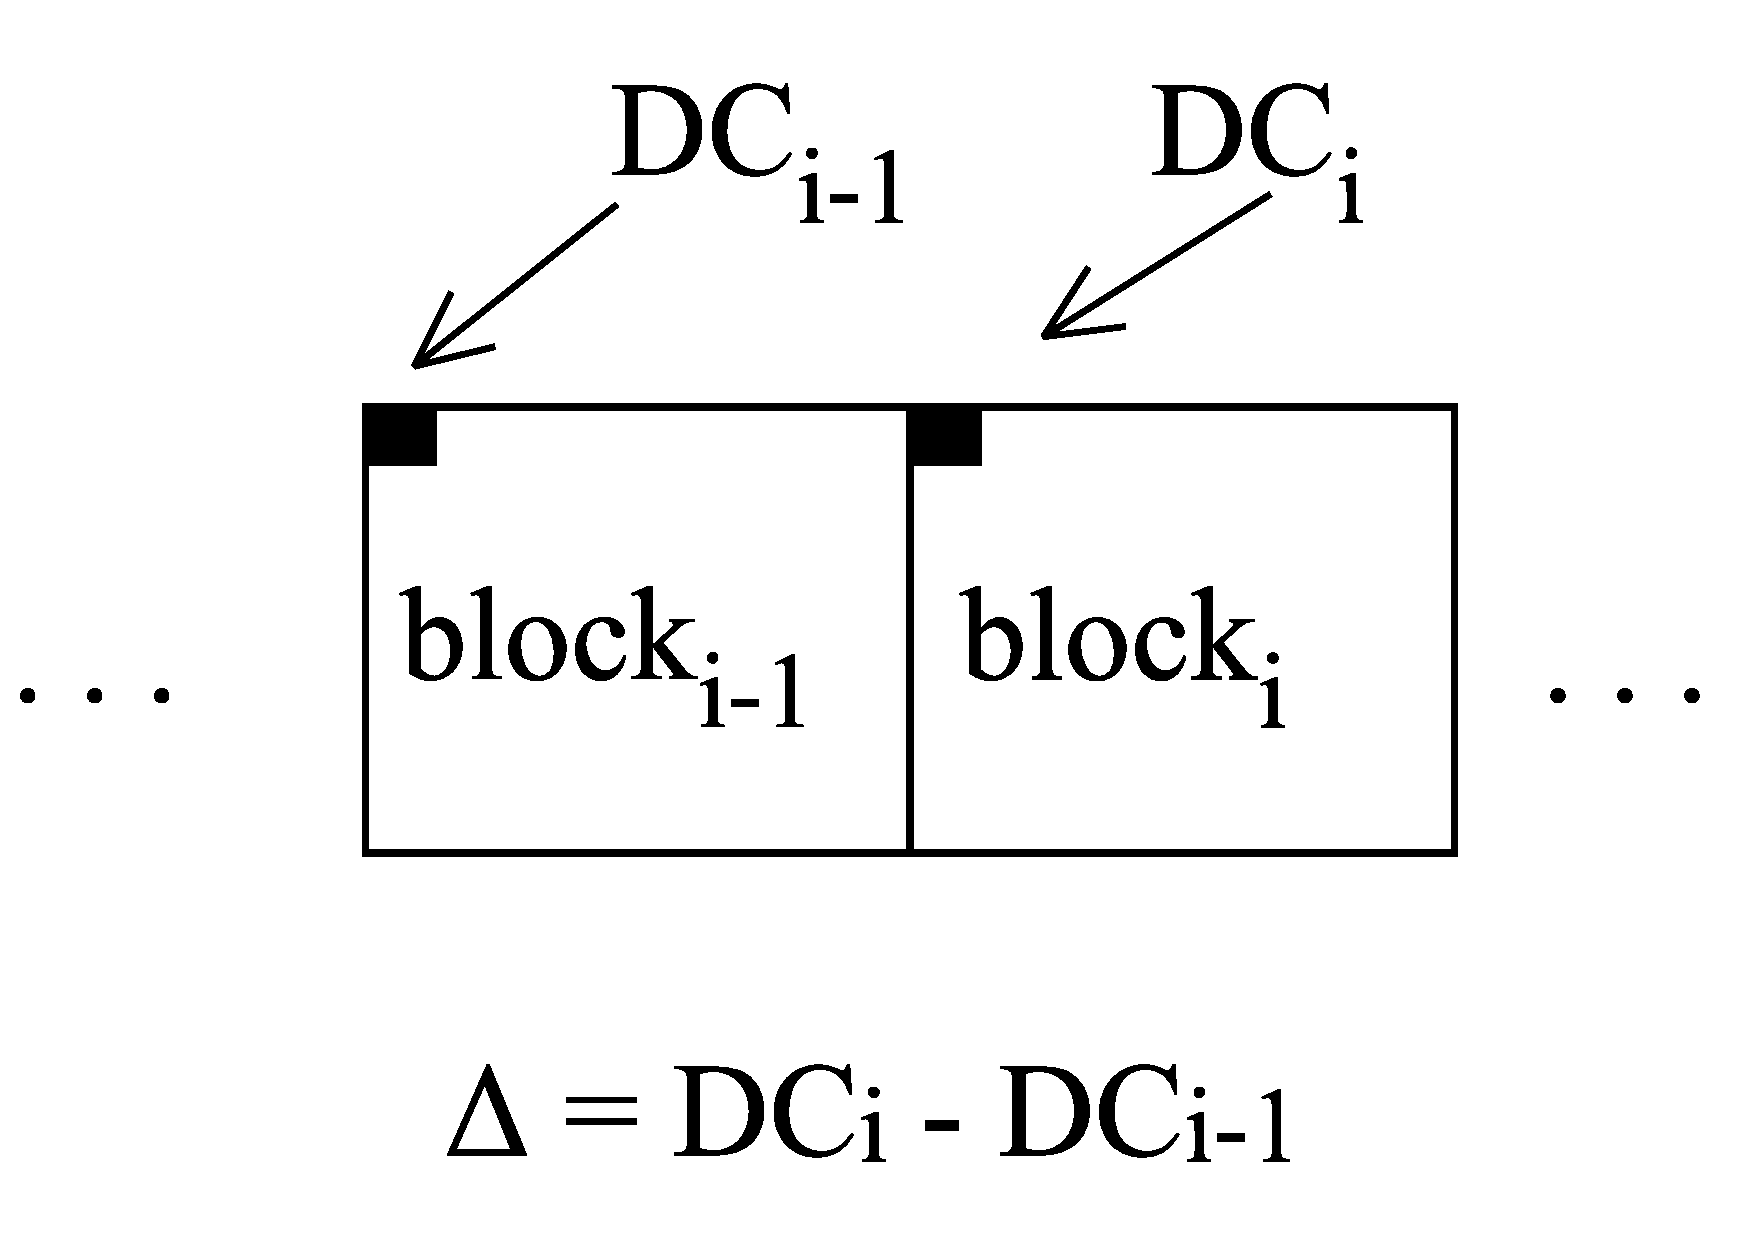
\includegraphics[width=0.3\textwidth]{slike/Diferencialno_kodiranje_DC.pdf}
\end{center}
\caption{Diferencialno DC kodiranje. Vir:~\cite{wallace1992jpeg}.}
\label{Diferencialno_kodiranje_DC}
\end{figure}
Obravnavanje DC koeficientov ločeno je smiselno, ker vsebujejo večino informacij na sliki. \par
Preostanejo AC koeficienti, ki jih najprej preuredimo v enovrstično zaporedje po principu prikazanem na Sliki \ref{zig_zag_zaporedje}. S to razporeditvijo skupaj združimo koeficiente, ki predstavljajo nižje frekvence. Koeficienti na začetku zaporedja imajo večjo verjetnost, da so neničelni. To je koristno za entropijsko kodiranje (\textit{angl.} entropy coding), ki ga bomo izvedli na teh zaporedjih.\par
\begin{figure}[ht] % vir (https://www.ijg.org/files/Wallace.JPEG.pdf)
\begin{center}
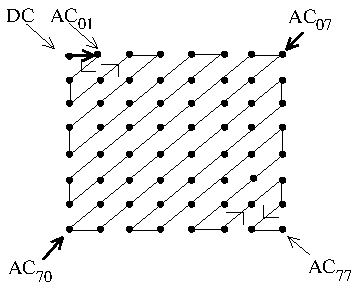
\includegraphics[width=0.5\textwidth]{slike/zig_zag_zaporedje.pdf}
\end{center}
\caption{Zaporedje kodiranje AC koeficientov. Vir: ~\cite{wallace1992jpeg}.}
\label{zig_zag_zaporedje}
\end{figure}
Sedaj imamo zaporedje 63 AC koeficientov, ki jih lahko dalje preoblikujemo.\par
Zadnji korak kodiranja JPEG-a je entropijsko kodiranje. Tukaj se izvede kompresija podatkov brez izgub. Uporabijo se statistične lastnosti kvantiziranih koeficientov DCT. V JPEG standardu sta predloženi dve metodi entropijskega kodiranja, to sta Huffmanovo kodiranje in aritmetično kodiranje. Tukaj bomo opisali zgolj Huffmanovo kodiranje, saj se to uporablja v privzetem kodeku.\par
Preden lahko uporabimo Huffmanovo kodiranje moramo pripraviti podatke v primerno obliko.
Nato se na teh podatkih lahko izvede Huffmanovo kodiranje. Pri tem kodiranju potrebujemo tabele za kodiranje, ki jih kasneje potrebujemo tudi pri dekodiranju. Te tabele niso specificirane v standardu. Tu je pri aplikacijah več izbir, lahko se uporablja ista tabela za vse slike, lahko se pa te tabele dinamično izračunajo pred kodiranjem slike. Kot možna izbira je v JPEG standardu podana ena tabela za DC koeficiente in ena tabela za AC koeficiente. JPEG omogoča sicer uporabo različnih tabel za različne barvne kanale, vendar dovoljeni sta največ dve DC tabeli in dve AC tabeli.\par
Najprej naredimo vmesno predstavitev za AC koeficiente. Zapisali jih bomo kot dve terke. Poimenujmo ju $S_1$ in $S_2$. V $S_1$ bomo zapisali dve števili. Prvo od teh števil bo predstavljalo število zaporednih ničel v našem zaporedju od prejšnjega neničelnega koeficienta. Drugo nam bo povedalo najmanjše število potrebnih bitov za predstavitev trenutnega AC koeficienta. $S_2$ bo vseboval vrednosti neničelnega AC koeficienta. Zapisali ju bomo kot $S_1 = (R, S)$ in $S_2 = (V)$.\par
Povedati moramo še nekaj omejitev teh koeficientov. $R$, ki predstavlja število zaporednih ničel lahko zavzame vrednosti od 0 do 15. V primeru, da je zaporednih več ničel zapišemo $S_1 = (15,0)$, s čimer povemo da imamo 16 zaporednih ničel. Dalje zapisujemo enako kot da bi bil 16. koeficient neničelno število. V najbolj ekstremnem primeru so lahko zapored trije zapisi (15,0), če imamo zapored 48 ničel. Vsakemu $S_1$ sledi v končnem zapisu en $S_2$. Edina izjema temu je, ko je zadnji 63. koeficient enak 0, kar se zgodi zelo pogosto. V tem primeru se zapiše za zadnji neničelen koeficient le $S_1$ z vsebino (0,0). V tem primeru se $S_2$ spusti. Torej $S_1 = (0,0)$ je oznaka za EOB (\textit{angl.} end of block), kar pomeni konec bloka.\par
Tukaj se ukvarjamo z 8 bitnimi števili v sliki pred transformacijami. Z nekaj numerične analize DCT ugotovimo, da se lahko DCT koeficienti povečajo kvečjemu za 3 bite. Kvantizacija tega ne poveča, saj lahko delimo zgolj s števili večjimi ali enakimi ena. Naš originalni interval števil je $\left[-2^7,2^7-1\right]$, torej so naši kvantizirani AC koeficienti kvečjemu znotraj $\left[-2^{10},2^{10}-1\right]$. Iz tega vidimo da bomo potrebovali za zapis $V$ v $S_2$ kvečjemu 10 bitov. Uporablja se zapis celih števil spremenljive dolžine (\textit{angl.} variable-length integer) kar bomo označili kot VLI. V tej obliki se lahko vsa števila iz zgornjega intervala zapišejo binarno z 1 do 10 biti. Torej bo $S$ v $S_1$ vsebovala števila od 1 do 10. Spremenljivko $S$ izračunamo s pomočjo Tabele \ref{tab:Velikost_AC}. Tukaj vrednost 0 ni mogoča, ker se vse ničle zapišejo z zaporedji ničel.\par

\begin{table}[ht]
\centering
\begin{tabular}{|c|c|c|}
\hline
$S$& AC koeficienti\\
\hline
 1& –1,1\\
 2& –3,–2,2,3\\
 3& –7..–4,4..7\\
 4& –15..–8,8..15\\
 5& –31..–16,16..31\\
 6& –63..–32,32..63\\
 7& –127..–64,64..127\\
 8& –255..–128,128..255\\
 9& –511..–256,256..511\\
10& –1 023..–512,512..1 023\\
\hline
\end{tabular}
\caption{Tabela za zapis velikosti AC koeficientov}
\label{tab:Velikost_AC}
\end{table}

Sedaj naredimo še vmesno predstavitev DC koeficientov. Pozorni moramo biti, da tukaj uporabljamo $\Delta = DC_i - DC_{i-1}$ in ne le trenutni koeficient DC. Ta predstavitev je zgrajena podobno kot pri AC koeficientih, ponovno imamo dve terki. V prvem je tokrat le $S_1 = (S)$, ker verjetnost, da dobimo 0 za razliko sosednjih DC koeficientov ni dovolj visoka, da bi se splačalo dodati vrednost za zaporedno število ničel. $S_2$ je podoben kot v prvem primeru. Razlika je, da so vrednosti razlike dveh DC koeficientov lahko na intervalu $\left[-2^{11},2^{11}-1\right]$, saj lahko pri razliki dveh 10 bitnih števil dobimo 11 bitno število. Za zapis $S$ uporabimo Tabelo \ref{tab:Velikost_DC}. Za razliko od primera za AC je tu vsebovana tudi 0, saj nismo ločeno obravnavali ničel. Na koncu je tudi dodatna vrstica zaradi možnosti večjih števil.\par
\begin{table}[ht]
\centering
\begin{tabular}{|c|c|c|}
\hline
$S$& vrednosti $\Delta$\\
\hline
 0& 0\\
 1& –1,1\\
 2& –3,–2,2,3\\
 3& –7..–4,4..7\\
 4& –15..–8,8..15\\
 5& –31..–16,16..31\\
 6& –63..–32,32..63\\
 7& –127..–64,64..127\\
 8& –255..–128,128..255\\
 9& –511..–256,256..511\\
10& –1 023..–512,512..1 023\\
11& –2 047..–1 024,1 024..2 047\\
\hline
\end{tabular}
\caption{Tabela za zapis velikosti DC koeficientov}
\label{tab:Velikost_DC}
\end{table}
Ko smo izračunali AC in DC koeficiente v vmesno predstavitev, lahko začnemo kodirati podatke v obliko za pošiljanje. $S_1$ se kodira s Huffmanovo kodo. Običajno so tabele za Huffmanovo kodo v naprej določene, lahko se pa računajo za vsako sliko posebej. V Tabeli \ref{tab:Huffman_AC_luminance} je prikazan izsek tabele, ki je podana v~\cite{ISO/IEC_10918-1} kot predlog za kodiranje svetilnosti AC koeficientov. Tukaj imamo zapisano zgolj za primera, ko je $R$ enak 0 ali 1. S pomočjo Huffmanovih tabel slikamo iz $S_1$ v neko binarno kodno besedo. Ta je lahko različnih dolžin. \par

\begin{table}[htbp]
\centering
\begin{tabular}{|c|c|c|}
\hline
$R$/$S$& Dolžina koda& Kodna beseda\\
\hline
0/0 (EOB) &4 &1010\\
0/1       &2 &00\\
0/2       &2 &01\\
0/3       &3 &100\\
0/4       &4 &1011\\
0/5       &5 &11010\\
0/6       &7 &1111000\\
0/7       &8 &11111000\\
0/8       &10 &1111110110\\
0/9       &16 &1111111110000010\\
0/A       &16 &1111111110000011\\
1/1       &4 &1100\\
1/2       &5 &11011\\
1/3       &7 &1111001\\
1/4       &9 &111110110\\
1/5       &11 &11111110110\\
1/6       &16 &1111111110000100\\
1/7       &16 &1111111110000101\\
1/8       &16 &1111111110000110\\
1/9       &16 &1111111110000111\\
1/A       &16 &1111111110001000\\
\hline
\end{tabular}
\caption{Izsek Huffmanove kodirne tabele za svetilnost AC koeficientov}
\label{tab:Huffman_AC_luminance}
\end{table}

$S_2$ bomo zapisali v obliki VLI. VLI je fiksno določen v standardu in ne moremo izbirati kakšno obliko uporabimo. Implementacija VLI v JPEG-u deluje na sledeč način. Recimo, da želimo število $n$ zakodirati. Če je $n \geq 0$ potem izračunamo njegovo binarno reprezentacijo. Iz te reprezentacije vzamemo $S$ najmanj pomembnih bitov (\textit{angl.} least significant bits), torej zadnjih $S$ bitov. Če je $n \leq 0$ potem izračunamo binarno reprezentacijo nepredznačenega n in vzamemo njen eniški komplement. Ponovno vzamemo $S$ najmanj pomembnih bitov od izračunanega eniškega komplementa. Ta proces naredimo, da učinkovito predstavimo koeficiente, ki vemo da so manjši od $2^{S}$. Lahko zapišemo tudi tabelo za izračun VLI, ki je prikazana v Tabeli \ref{tab:VLI_tabela}. Kasneje bomo na primeru pokazali kako se kodiranja več koeficientov združi zaporedno.
% razlaga kak variable length integerji(VLI) delujejo https://engineering.purdue.edu/~bouman/grad-labs/JPEG-Image-Coding/pdf/lab.pdf
% tabela za VLI na 33 slidu https://www.arl.wustl.edu/projects/fpx/workshop_0602/jpeg_recoder.pdf 
\begin{table}[ht]
\centering
\resizebox{\columnwidth}{!}{\begin{tabular}{|c|c|c|}
\hline
$S$& $V$& Predstavitev VLI\\
\hline
1  & -1,1 &0, 1\\
2  & -3,-2, 2, 3 &00, 01, 10, 11\\
3  & -7..-4, 4..7 &000..011, 100..111\\
4  & -15..-8, 8..15 &0000..0111, 1000..1111\\
5  & -31..-16, 16..31 &00000..01111, 10000..11111\\
6  & -63..-32, 32..63 &000000..011111, 100000..111111\\
7  & -127..-64, 64..127 &0000000..0111111, 1000000..1111111\\
8  & -255..-128, 128..255 &00000000..01111111, 10000000..11111111\\
9  & -511..-256, 256..511 &000000000..011111111, 100000000..111111111\\
10 & -1023..-512, 512..1023 &0000000000..0111111111, 1000000000..1111111111\\
11 & -2047..-1024, 1024..2047 &00000000000..01111111111, 10000000000..11111111111\\
\hline
\end{tabular}}
\caption{Reprezentacija celih števil v VLI}
\label{tab:VLI_tabela}
\end{table}

Sedaj bomo pokazali še kako se kodira DC koeficiente. Naprej kodiramo $S_1$. Ta je bolj enostaven kot v AC primeru, saj nimamo števila zaporednih ničel ($R$) in je kodirna tabela zato veliko manjša. Primer te tabele za svetilnost, ki je podan v~\cite{ISO/IEC_10918-1} je v Tabeli \ref{tab:Huffman_DC_luminance}. Za $S_2$ uporabimo enak način kodiranja z VLI kot pri AC koeficientih. Pri DC koeficientih pride sicer do specifičnega primera, kjer je koeficient, ki ga kodiramo 0. V tem primeru je $S = (0)$. Tukaj se $S_2$ praktično ne kodira oziroma nobenega števila ne dobimo od kodiranja. Dovolj informacij smo že zapisali s tem, da je $S = (0)$. 

\begin{table}[ht]
\centering
\begin{tabular}{|c|c|c|}
\hline
$S$&Dolžina koda&Kodna beseda\\
\hline
0&  2& 00\\
1&  3& 010\\
2&  3& 011\\
3&  3& 100\\
4&  3& 101\\
5&  3& 110\\
6&  4& 1110\\
7&  5& 11110\\
8&  6& 111110\\
9&  7& 1111110\\
10& 8& 11111110\\
11& 9& 111111110\\
\hline
\end{tabular}
\caption{Huffmanova kodirna tabela za svetilnost DC koeficientov}
\label{tab:Huffman_DC_luminance}
\end{table}

\section{Kvaliteta kompresiranih slik}
Opisali bomo nekaj okvirnih pravil za kompresijo pri določeni kvaliteti. Če imamo barvno sliko z srednje zahtevnimi oblikami velja:
\begin{itemize}
   \item 0,25 - 0,5 bitov na piksel nam prinese srednjo do dobro kvaliteto. Je primerno za nekatere aplikacije.
   \item 0,5 - 0,75 bitov na piksel nam prinese dobro do zelo dobro kvaliteto. Je primerno za veliko aplikacij.
   \item 0,75 - 1,5 bitov na piksel nam prinese odlično kvaliteto. Je primerno za večino aplikacij.
   \item 1,5 - 2 bita na piksel nam prinese skoraj neločljivo kvaliteto od originala. Primerno za najbolj zahtevne aplikacije
\end{itemize}
Te mere večino časa držijo, a na njih se ne moramo zanesti. JPEG ni format kjer bi pri kompresiji določili količino prostora za shranjevanje slike. Navedemo nivo kvalitete, ki ga želimo in nam vrne sliko s potrebno količino podatkov, da to dosežemo.

\section{Primer kodiranja}\label{Primer_kodiranja}
Podajmo najprej nek blok slike $I$

\begin{gather*}
 I =
  \begin{bmatrix}
 182& 161& 152& 164& 165& 171& 188& 191\\
 160& 157& 169& 176& 179& 177& 181& 189\\
 173& 176& 179& 180& 187& 182& 169& 175\\
 190& 186& 183& 176& 182& 184& 169& 164\\
 185& 195& 189& 178& 176& 183& 180& 167\\
 185& 190& 189& 185& 177& 175& 177& 170\\
 184& 171& 182& 185& 180& 174& 172& 174\\
 175& 186& 179& 178& 180& 182& 181& 184\\
   \end{bmatrix}.
\end{gather*}
Zamaknimo to za $2^7$ na interval $\left[-2^{7},2^{7}-1\right]$
\begin{gather*}
 I - 128 =
  \begin{bmatrix}
  54& 33& 24& 36& 37& 43& 60& 63\\
  32& 29& 41& 48& 51& 49& 53& 61\\
  45& 48& 51& 52& 59& 54& 41& 47\\
  62& 58& 55& 48& 54& 56& 41& 36\\
  57& 67& 61& 50& 48& 55& 52& 39\\
  57& 62& 61& 57& 49& 47& 49& 42\\
  56& 43& 54& 57& 52& 46& 44& 46\\
  47& 58& 51& 50& 52& 54& 53& 56\\
   \end{bmatrix}.
\end{gather*}
Izračunajmo DCT tega bloka

\begin{gather*}
 C(I) =
  \begin{bmatrix}
 399,1&   3,5&  -0,7&   4,2&   0,9&   0,3&   1,8&   0 \\
 -20,6& -27,3&   9,3&   6,1&   9,8&   2,3&   1,1&   1 \\
 -15,1& -35 &  15,4&  -4,2&  14,7&   5,6&  -3,1&  -0,5\\
  -2,7&   3,8&  15,3&  -0,6&  -0,9&  12 &  -5,2&   0,3\\
   3,4&   4,7&  16,6&  10 &  -8,9&  -1,9&  -4 &  -2,8\\
  -4,8&  10,9&   3,4&   9,1&  10,1&   4,1&   4,1&   1,1\\
   5 &   5,7&   3,9&   0,3&  -3,3&  -4,4&  -4,6&  -2,5\\
   0,2&  -0,4&  0 &   0,3&  -0,2&  0 &  0 &  -0,3\\
   \end{bmatrix}
\end{gather*}
Sedaj še kvantiziramo ta blok s kvantizacijsko tabelo za svetilnost prikazano v Tabeli \ref{tab:Kvantizacija_svetilnost} in dobimo

\begin{gather*}
 C^Q(I) =
  \begin{bmatrix}
 25&  0&  0&  0&  0&  0&  0&  0\\
 -2& -2&  1&  0&  0&  0&  0&  0\\
 -1& -3&  1&  0&  0&  0&  0&  0\\
  0&  0&  1&  0&  0&  0&  0&  0\\
  0&  0&  0&  0&  0&  0&  0&  0\\
  0&  0&  0&  0&  0&  0&  0&  0\\
  0&  0&  0&  0&  0&  0&  0&  0\\
  0&  0&  0&  0&  0&  0&  0&  0\\
   \end{bmatrix}
\end{gather*}
To zapišemo v enovrstično zaporedje po Sliki \ref{zig_zag_zaporedje}. Torej ločeno zapišemo DC koeficient in 63 AC koeficientov. Velja, da je DC = 25 in

\begin{gather*}
 \hbox{AC} =
  \begin{array}{*{16}c}
    [0,& -2,& -1,& -2,& 0,& 0,& 1,& -3,& 0,& 0,& 0,& 1,& 0,& 0,& 0,& 0,\\
    0,&  1,&  0,&  0,& 0,& 0,& 0,&  0,& 0,& 0,& 0,& 0,& 0,& 0,& 0,& 0,\\
    0,&  0,&  0,&  0,& 0,& 0,& 0,&  0,& 0,& 0,& 0,& 0,& 0,& 0,& 0,& 0,\\
    0,&  0,&  0,&  0,& 0,& 0,& 0,&  0,& 0,& 0,& 0,& 0,& 0,& 0,& 0& ].\\
  \end{array}
\end{gather*}
Sedaj, ko imamo koeficiente v pravilnem zaporedju jih zapišemo v vmesni predstavitvi. Tukaj bomo računali kot da je to prvi blok slike, torej je prejšnji DC koeficient enak 0. Najprej izračunamo $\Delta = 25-0 = 25$. Iz Tabele \ref{tab:Velikost_DC} razberemo, da je $S = 5$, torej bo vmesna predstavitev DC koeficienta (5)(25). \par
Pretvorimo še AC koeficiente v vmesno predstavitev. Prvi člen je 0 zato bo $R = 1$. Drugi člen je -2, zapišemo po Tabeli \ref{tab:Velikost_AC}, da je $S = 2$, torej dobimo zapis (1,2)(-2). Podobno nadaljujemo in dobimo celo zaporedje terk bloka kot
\begin{equation*}
  \begin{aligned}
    &(5)(25),\;(1,2)(-2),\;(0,1)(-1),\;(0,2)(-2),\\
    &(2,1)(1),\;(0,2)(-3),\;(3,1)(1),\;(5,1)(1),\;(0,0)
  \end{aligned}
\end{equation*}
Sedaj začnemo dejansko kodirat v zapis za pošiljanje. Najprej začnemo z DC koeficientom, kjer po Tabeli \ref{tab:Huffman_DC_luminance} (5) preslikamo v 110. Nato po VLI preslikamo (25). Najprej zapišemo binarno reprezentacijo, ki je 00011001. Uporabimo $S$ najmanj pomembnih bitov, torej v tem primeru 5 bitov. Ostane nam 11001. Tukaj uporabljamo 8-bitno reprezentacijo. V splošnem je potrebna 16-bitna reprezentacija, da zadostimo vsem možnim številom. To dvoje damo zapored in dobimo kodiranje 11011001 za DC koeficient.\par
Nadaljujemo z AC koeficienti. Najprej bomo poiskali vse pretvorbe za $S_1$ v razširjeni tabeli \ref{tab:Huffman_AC_luminance} iz~\cite{ISO/IEC_10918-1}. 
\begin{equation*}
  \begin{aligned}
    &(1,2)\indent 11011   \\
    &(0,1)\indent 00   \\
    &(0,2)\indent 01   \\
    &(2,1)\indent 11100   \\
    &(3,1)\indent 111010   \\
    &(5,1)\indent 1111010   \\
    &(0,0)\indent 1010 
  \end{aligned}
\end{equation*}
Pretvorimo še vse $S_2$ po VLI. Najprej pretvorimo -2, kjer zapišemo 2 v binarni reprezentaciji 00000010, naredimo eniški komplement, to je 11111101. Vzamemo njenih $S$ najmanj pomembnih bitov, torej 2 bita in dobimo 01. Podobno naredimo za ostala števila
\begin{alignat*}{2}
    &(-2) \indent && 01 \\
    &(-1) \indent && 0 \\
    &(1)  \indent && 1 \\ 
    &(-3) \indent && 00 
\end{alignat*}
Sedaj po vrsti uporabimo izračunano
\begin{alignat*}{2}
    &(5)(25),  \indent  &&110\;11001\\
    &(1,2)(-2) \indent  &&11011\;01\\
    &(0,1)(-1) \indent  &&00\;0\\
    &(0,2)(-2) \indent  &&01\;01\\
    &(2,1)(1)  \indent  &&11100\;1\\
    &(0,2)(-3) \indent  &&01\;00\\
    &(3,1)(1)  \indent  &&111010\;1\\
    &(5,1)(1)  \indent  &&1111010\;1\\
    &(0,0)     \indent  &&1010
\end{alignat*}
Sedaj to zaporedno skupaj napišemo v en binaren niz (presledki so dodani za lažje branje) 
\begin{equation*}
11011001\;11011010\;00010111\;10010100\;11101011\;11101011\;010
\end{equation*}
Tako smo uspeli cel 8x8 blok zakodirat v 51 bitov. Blok vsebuje 64 pikslov, vsak od teh je vseboval 8 bitov informacije. Torej smo uspeli zmanjšati podatke iz 512 bitov na 51 bitov. V tem primeru smo stisnili podatke za 10-krat. O dejanskem prihranku na sliki tukaj ne moramo povedati veliko, saj rabimo vzorec več blokov in tukaj smo delali le na barvnem kanalu za svetilnost. Če gledamo le sliko v sivinah smo sicer dosegli kompresijo na 0,8 bitov na piksel.


\section{Dekodiranje}
Pokazali bomo še kako pridemo iz kodiranega zaporedja bitov nazaj do slike, ki je blizu originalu.\par
Shema kako poteka dekodiranje je prikazana na Sliki \ref{Shema_dekodiranja_JPEG}. Prvi korak je entropijsko dekodiranje, kjer moramo tabele za dekodiranje prebrat iz glave JPEG-a. Mi delamo s Huffmanovimi kodi. Nato preoblikujemo nazaj izhod iz Huffmanovega dekodiranja nazaj v 8x8 blok. Ta gre skozi dekvantiziranje s pomočjo tabel, ki so zapisane v glavi JPEG-a. Na tej tabeli izvedemo inverzni DCT, ki nam da končen blok. V primeru več barvnih kanalov moramo istoležne bloke nazaj združiti v naš približek originalne slike.\par
\begin{figure}[ht] % vir (https://www.w3.org/Graphics/JPEG/itu-t81.pdf)
\begin{center}
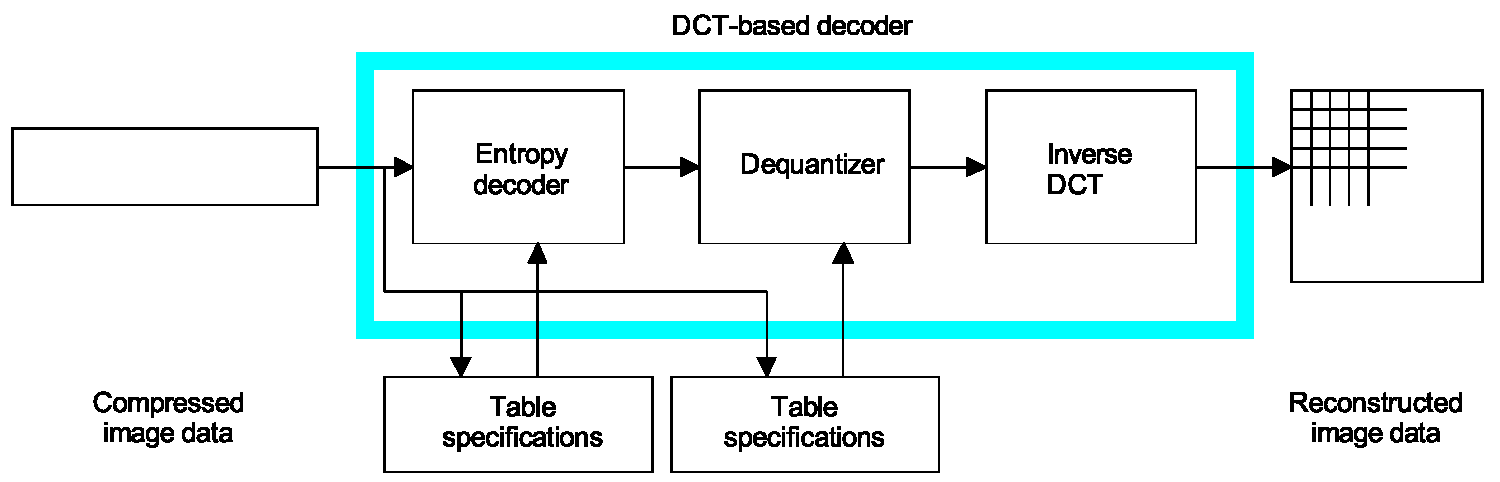
\includegraphics[width=0.9\textwidth]{slike/Shema_Inverz_JPEG.pdf}
\end{center}
\caption{Shema dekodiranja JPEG-a. Vir:~\cite{ISO/IEC_10918-1}}
\label{Shema_dekodiranja_JPEG}
\end{figure}

Imamo podan binaren niz bloka. V tem nizu ne vemo kako dolga je kodirna beseda za $S_1$. Tukaj potrebujemo lastnost Huffmanovega koda, da lahko beremo bite po vrsti, da dobimo zakodiran simbol. Da lahko to naredimo, moramo iz tabele, ki smo jo prebrali v glavi JPEG-a, zgraditi dvojiško drevo. To drevo zgleda tako, da če po vrsti beremo bite vsaka 0 pomeni, da gremo levo po drevesu, vsaka 1 pomeni, da gremo desno po drevesu. To deluje, ker so Huffmanovi kodi tako zgrajeni, da nobena kodirna beseda ne mora biti prefiks drugi daljši kodirni besedi.\par
Prvi simbol se nanaša na DC koeficient, zato prvo uporabimo zgrajeno drevo za tabelo DC koeficientov. V našem primeru je to za Tabelo \ref{tab:Huffman_DC_luminance}. Torej, ko beremo binarni niz ga porabimo tako dolgo, da pridemo do lista. Sedaj smo dobili $S_1 = (S)$. Dobili smo informacijo, da naslednjih $S$ bitov predstavlja razliko DC koeficientov. Torej vzamemo naslednjih $S$ bitov, ki so števila zakodirana po VLI. Da pridemo iz VLI do celih števil uporabimo naslednjo proceduro.\par
Označimo bitno zaporedje z $b$, kjer je $b_i$ i-ti člen tega zaporedja. Definirajmo funkcijo binToInt kot funkcijo, ki preslika binarno število v celo število. 
\begin{itemize}
  \item Če je $b_0 = 0$, potem vemo, da je to negativno število. V tem primeru moramo izračunati eniški komplement $b$ in ga označimo z $b'$. Dobimo $\Delta = -\hbox{binToInt}(b')$. 
  \item Če je $b_0 = 1$, potem vemo, da je to pozitivno število. V tem primeru je $\Delta = \hbox{binToInt}(b)$. 
\end{itemize}
Da dobimo originalen DC koeficient moramo še izračunati $DC_i = \Delta + DC_{i-1}$, torej odštejemo še prejšnji DC koeficient. Če je ta blok prvi, potem odštejemo 0. Število $DC_i$ damo na svoje mesto levo zgoraj v 8x8 bloku.\par
Sledijo zakodirani vsi AC koeficienti. Te bomo zaporedoma zapisovali v seznam dokler jih ne bo 63. Podobno kot v DC primeru začnemo brati binarni niz, vendar sedaj uporabimo zgrajeno drevo za tabelo AC koeficientov. Ta je v našem primeru \ref{tab:Huffman_AC_luminance}. Beremo binarni niz dokler ne pridemo do lista v drevesu. Ko pridemo do lista dobimo zakodirano $S_1 = (R, S)$. Kjer $R$ pomeni število ničel v zaporedju. Tukaj moramo obravnavati nekaj primerov:
\begin{itemize}
  \item Če je $R = 0$ in $S = 0$, potem smo prišli do EOB in moramo naš seznam AC koeficientov napolniti s toliko ničlami, da bo vseboval 63 števil.
  \item Če je $R = 15$ in $S = 0$, moramo v seznam AC koeficientov zapisati 16 ničel.
  \item V vseh ostalih primerih zapišemo v seznam AC koeficientov $R$ ničel. Nato vzamemo naslednjih $S$ bitov, ki predstavljajo zakodirano število po VLI. To število dekodiramo na isti način kot je bilo opisano pri DC koeficientu in ga dodamo na seznam. 
\end{itemize}
Do konca bloka pridemo v primeru, ko je $R = 0$ in $S = 0$ ali ko imamo v seznamu zapisanih 63 koeficientov. Če še nismo na koncu bloka ponovimo postopek za naslednji koeficient.\par
Na koncu tega postopka smo dobili seznam 63 AC koeficientov, te moramo razporediti nazaj v blok 8x8. To storimo na enak način, kot pri kodirali le, da tokrat dodajamo koeficiente po vrstnem redu na Sliki \ref{zig_zag_zaporedje}.\par
Sedaj ko imamo vse koeficiente zapisane v bloku jih moramo še dekvantizirati. To poteka tako, da preberemo tabelo za kvantiziranje iz glave JPEG-a. V našem primeru je to Tabela \ref{tab:Kvantizacija_svetilnost} za svetilnost. Približke originalnim DCT koeficientom izračunamo po naslednji formuli:
\begin{equation}
C'(u,v) = C^Q(u,v) \cdot Q(u,v).
\label{eq:dekvantizacija}
\end{equation}
To storimo za vse $u,v = 0,\ldots,7$.\par
Na tej tabeli se sedaj izvede inverzni DCT. Koeficientom, ki smo jih dobili moramo še prišteti zamik, da bodo ponovno na intervalu $\left[0,2^P-1\right]$. Označimo s $\widetilde{z}'$ zamaknjen približek piksla. Potem je $\widetilde{z} = \widetilde{z}' + 2^{P-1}$ naš končen približek piksla.\par
Če osnovna resolucija slike ni bila deljiva z 8, moramo tu odstranit piksle, ki smo jih v tistem koraku dodali.
V primeru, da smo imeli sliko z več barvnimi kanali in smo uporabili barvno podvzorčenje moramo še uporabiti metode, da kanale ki predstavljajo barvo razširimo nazaj na originalno velikost.

\section{Primer dekodiranja}
Sedaj bomo dekodirali blok, ki smo ga v poglavju \ref{Primer_kodiranja} zakodirali. Dano imamo torej bitno zaporedje
\begin{equation*}
11011001\;11011010\;00010111\;10010100\;11101011\;11101011\;010
\end{equation*}
Če si izrišemo graf za Tabelo \ref{tab:Huffman_DC_luminance} vidimo, da 110 pripada $S_1 = (5)$. Iz tega vidimo, da moramo vzeti naslednjih 5 bitov za DC koeficient. Dobili smo 11001, ki je v obliki VLI in ga pretvorimo nazaj v celo število. Vidimo, da ima $b_0=1$, torej je pozitivno število in 11001 samo pretvorimo v celo število, ki je 25. Sedaj moramo še prišteti prejšnji DC koeficient, ki je bil 0, ker smo to vzeli za prvi blok. Torej je naš DC koeficient DC $= 25+0 = 25$.\par
Nadaljujemo z AC koeficienti. Izrišemo si graf za celo razširjeno Tabelo \ref{tab:Huffman_AC_luminance} iz~\cite{ISO/IEC_10918-1}. Dobimo 11011, ki pripada $S_1 = (1, 2)$. Prvo zapišemo eno ničlo v zaporedje. Nato vzamemo naslednja dva bita 01 in dobimo koeficient 1. Nadaljujemo in dobimo 00, ki gre v $S_1 = (0, 1)$, vzamemo en bit, ki je 0 in to pomeni -1. Zapišemo te dve in vse nadaljnje spodaj

\begin{alignat*}{5}
&\hbox{Huffmanove besede}\;\; && (R,S)\;\; \hbox{VLI}&&\indent\;\;  V&&\indent && \hbox{Dodani koeficienti}\\
    &11011   &&(1,2)\indent01&&\indent -2&&\indent &&0,\;-2            \\
    &00      &&(0,1)\indent 0&&\indent -1&&\indent &&-1               \\
    &01      &&(0,2)\indent01&&\indent -2&&\indent &&-2               \\
    &11100   &&(2,1)\indent 1&&\indent  1&&\indent &&0,\;0,\;1          \\
    &01      &&(0,2)\indent00&&\indent -3&&\indent &&-3               \\
    &111010  &&(3,1)\indent 1&&\indent  1&&\indent &&0,\;0,\;0,\;1       \\
    &1111010 &&(5,1)\indent 1&&\indent  1&&\indent &&0,\;0,\;0,\;0,\;0,\;1 \\
    &1010    &&(0,0)\indent  &&\indent   &&\indent &&46\hbox{-krat } 0
\end{alignat*}
Dobimo DC =  25 in
\begin{gather*}
 \hbox{AC} =
  \begin{array}{*{16}c}
    [0,& -2,& -1,& -2,& 0,& 0,& 1,& -3,& 0,& 0,& 0,& 1,& 0,& 0,& 0,& 0,\\
     0,&  1,&  0,&  0,& 0,& 0,& 0,&  0,& 0,& 0,& 0,& 0,& 0,& 0,& 0,& 0,\\
     0,&  0,&  0,&  0,& 0,& 0,& 0,&  0,& 0,& 0,& 0,& 0,& 0,& 0,& 0,& 0,\\
     0,&  0,&  0,&  0,& 0,& 0,& 0,&  0,& 0,& 0,& 0,& 0,& 0,& 0,& 0 & ],\\
  \end{array}
\end{gather*}
kar je enako kot smo zakodirali.\par
Sedaj, ko imamo to zaporedje ga zapišemo nazaj v 8x8 blok po Sliki \ref{zig_zag_zaporedje}. Dobimo nazaj naslednji 8x8 blok
\begin{gather*}
 C^Q(I) =
  \begin{bmatrix}
 25&  0&  0&  0&  0&  0&  0&  0\\
 -2& -2&  1&  0&  0&  0&  0&  0\\
 -1& -3&  1&  0&  0&  0&  0&  0\\
  0&  0&  1&  0&  0&  0&  0&  0\\
  0&  0&  0&  0&  0&  0&  0&  0\\
  0&  0&  0&  0&  0&  0&  0&  0\\
  0&  0&  0&  0&  0&  0&  0&  0\\
  0&  0&  0&  0&  0&  0&  0&  0\\
   \end{bmatrix}.
\end{gather*}
Ta blok moramo sedaj dekvantizirati po \eqref{eq:dekvantizacija} s Tabelo \ref{tab:Kvantizacija_svetilnost}, saj smo to tabelo uporabili za kvanztizacijo.
\begin{gather*}
 \widetilde{C}(I) =
  \begin{bmatrix}
400&   0&   0&   0&   0&   0&   0&   0\\
-24& -24&  14&   0&   0&   0&   0&   0\\
-14& -39&  16&   0&   0&   0&   0&   0\\
  0&   0&  22&   0&   0&   0&   0&   0\\
  0&   0&   0&   0&   0&   0&   0&   0\\
  0&   0&   0&   0&   0&   0&   0&   0\\
  0&   0&   0&   0&   0&   0&   0&   0\\
  0&   0&   0&   0&   0&   0&   0&   0\\
   \end{bmatrix}.
\end{gather*}
Na tej matriki naredimo sedaj inverzni DCT, kjer rezultat zaokrožimo na najbližje celo število. Dobimo
\begin{gather*}
 \widetilde{I}-128 =
  \begin{bmatrix}
  40& 36& 31& 30& 36& 47& 60& 69\\
  40& 40& 39& 41& 44& 49& 54& 57\\
  44& 47& 51& 53& 53& 50& 46& 44\\
  54& 56& 58& 59& 56& 49& 43& 38\\
  62& 61& 59& 56& 52& 48& 44& 42\\
  62& 60& 56& 53& 50& 49& 48& 48\\
  54& 54& 53& 53& 53& 52& 51& 51\\
  45& 48& 52& 55& 56& 55& 53& 51\\
  \end{bmatrix}.
\end{gather*}
Ta približek je še zamaknjen za $2^7$, zato še to prištejemo in dobimo končni približek originalnemu bloku
\begin{gather*}
 \widetilde{I} =
  \begin{bmatrix}
  168& 164& 159& 158& 164& 175& 188& 197\\
  168& 168& 167& 169& 172& 177& 182& 185\\
  172& 175& 179& 181& 181& 178& 174& 172\\
  182& 184& 186& 187& 184& 177& 171& 166\\
  190& 189& 187& 184& 180& 176& 172& 170\\
  190& 188& 184& 181& 178& 177& 176& 176\\
  182& 182& 181& 181& 181& 180& 179& 179\\
  173& 176& 180& 183& 184& 183& 181& 179\\
  \end{bmatrix}.
\end{gather*}
Originalen blok zgleda sledeče
\begin{gather*}
 I =
  \begin{bmatrix}
 182& 161& 152& 164& 165& 171& 188& 191\\
 160& 157& 169& 176& 179& 177& 181& 189\\
 173& 176& 179& 180& 187& 182& 169& 175\\
 190& 186& 183& 176& 182& 184& 169& 164\\
 185& 195& 189& 178& 176& 183& 180& 167\\
 185& 190& 189& 185& 177& 175& 177& 170\\
 184& 171& 182& 185& 180& 174& 172& 174\\
 175& 186& 179& 178& 180& 182& 181& 184\\
   \end{bmatrix}.
\end{gather*}
Če izračunamo razliko vidimo do koliko napake je prišlo
\begin{gather*}
 I - \widetilde{I}=
  \begin{bmatrix}
 14&  -3&  -7&   6&   1&  -4&   0&  -6\\
 -8& -11&   2&   7&   7&   0&  -1&   4\\
  1&   1&   0&  -1&   6&   4&  -5&   3\\
  8&   2&  -3& -11&  -2&   7&  -2&  -2\\
 -5&   6&   2&  -6&  -4&   7&   8&  -3\\
 -5&   2&   5&   4&  -1&  -2&   1&  -6\\
  2& -11&   1&   4&  -1&  -6&  -7&  -5\\
  2&  10&  -1&  -5&  -4&  -1&   0&   5\\
   \end{bmatrix}.
\end{gather*}
Vidimo, da je najvišja razlika med originalom in približkom 14, kar ni veliko. Ta bloka sta in njuna razlika so prikazani na Sliki \ref{kodiranje_dekodiranje_napaka}.

\begin{figure}[ht] % vir generirano z mojo kodo
\begin{center}
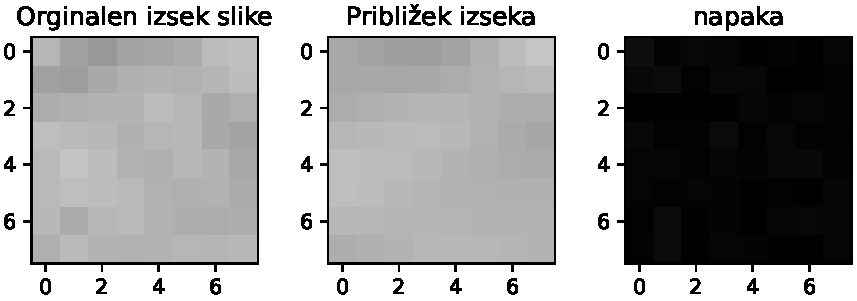
\includegraphics[width=0.9\textwidth]{slike/izsek_primerjava_napaka_Primera.pdf}
\end{center}
\caption{Prikaz napake po kodiranju z JPEG-om. Levo je prikazan originalen blok, na sredini je blok po rekonstrukciji in na desni je njuna razlika. Vir:.}%vir je moja koda
\label{kodiranje_dekodiranje_napaka}
\end{figure}


%\section{Slabosti diskretne kosinusne transformacije}


\chapter{Uporaba diskretne kosinusne transformacije}
\label{Uporaba_DCT}
V tem poglavju si bomo pogledali dejansko uporabo DCT v kombinaciji z JPEG standardom. Ovrednotili bomo kvaliteto slik s pomočjo PSNR (\textit{angl.} Peak signal-to-noise ratio).
\section{Slike}
Ogledali si bomo tri slike, ki jih bomo nato pretvorili v JPEG s 5 različnimi nivoji kvalitete. Pretvarjali jih bomo s knjižnico PIL v programskem jeziku Python. Za te različne kvalitete bomo nastavili spremenljivko \textit{quality} v funkciji \textit{save} na 5 različnih vrednosti. Izbrali smo vrednosti 5, 25, 50, 75 in 95.\par
Za mero kakovosti slik bomo uporabili mero PSNR, ki meri razmerje med največjo možno močjo signala in močjo nezaželenega šuma. PSNR je definirana v~\cite{psnr} kot
\begin{equation}
    \hbox{PSNR}(X, \widetilde{X}) = 10\log_{10}\frac{255^2}{\hbox{MSE}(X, \widetilde{X})}
\label{eq:psnr}
\end{equation}
Tukaj je z $X$ označena originalna slika in z $\widetilde{X}$ kompresiran približek $X$. Za funkcijo MSE je uporabljena ista definicija kot v \ref{eq:MSE}. Enota PSNR je $dB$. Ta definicija je zapisana za primer, ko imamo 8-bitno sliko, torej je možnih 255 pozitivnih vrednosti piksla. V drugih primerih je potrebno prilagoditi definicijo številu bitov. Pri slikah v sivinah je ta definicija enolična. Ko gledamo PSNR na barvnih slikah sta dve možni definiciji. Razlika je pri tem kako izračunamo MSE. Lahko vzamemo povprečje MSE na treh barvnih kanalih ali izračunamo MSE na svetilnosti, torej na Y komponenti, če imamo sliko zapisamo v Y'C\textsubscript{B}C\textsubscript{R}. Mi bomo tu uporabljali definicijo, kjer vzamemo povprečje treh barvnih kanalov.\par
Ko gledamo vrednosti PSNR nam višje vrednosti predstavljajo boljšo kvaliteto. V splošnem velja, da za 8-bitne slike je PSNR nad 25 že običajno soliden, nad 30 pa zelo dober.\par
Izbrali smo tri slike, ki se pogosto uporabljajo v procesiranju slik. Te slike imajo resolucijo 512x512 in imajo tri barvne kanale. Njihovi originali so v formatu TIFF. Obstajajo sicer formati, ki hranijo sliko brez izgube kvalitete, ki zavzamejo manj prostora kot TIFF, vendar je vseeno široko uporabljan.
\begin{comment}
\begin{figure}[ht] % vir python
\begin{center}
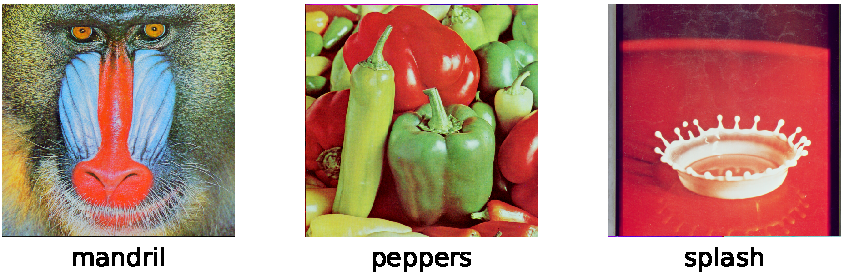
\includegraphics[width=0.9\textwidth]{slike/Original_mandril_lena_peppers.pdf}
\end{center}
\caption{Slike uporabljene za testiranje JPEG-a. Imena slik so napisana pod njimi.}
\label{Original_mandril_lena_peppers}
\end{figure}
\end{comment}
Te slike smo pretvorili v JPEG s petimi različnimi nivoji kvalitete in izračunali njihov PSNR. Za sliko mandril bodo kvalitete prikazane na Slike \ref{Quality_mandril} in PSNR ter velikosti datotek v Tabeli \ref{tab:mandril_psnr}. Podobno imamo za sliko peppers na Sliki \ref{Quality_peppers} in v Tabeli \ref{tab:peppers_psnr} ter za sliko splash na Sliki \ref{Quality_splash} in v Tabeli \ref{tab:splash_psnr}. \par
Poglejmo sedaj kaj ti rezultati pomenijo. Opazimo, da imajo originali PSNR = $\infty$, to se zgodi ker je MSE slike same s sabo enak 0. Velikost datotek originalov je tudi v vseh primerih enak, saj so vse slike dimenzij 512x512 in imajo tri barvne kanala, vsak po 8 bitov. Ker tu ni uporabljena nobena kompresija so slike enake velikosti.\par
V splošnem velja pravilo, da pri izbiri kvalitete 95 je skoraj neopazna izguba kvalitete slike. Privzeta izbira v tej implementaciji je sicer 75, kar je tudi zelo težko opazno. Kvalitete manjše od 50 imajo običajno že vidne artefakte kompresije. Te bi se naj uporabljajo zgolj za aplikacije, kjer je mala velikost slik zares nujna. Tukaj moramo biti tudi pazljivi, saj JPEG dobro deluje na naravnih oblikah, ki jih dobimo s slikanjem okolice. Zlahka se da generirati umetno sliko, kjer bodo pri visokih kvalitetah že vidni artefakti na robovih.\par
Nivo kompresije JPEG-a je že pri izbiri kvalitete 95 zelo dober. Na primerih nam to prinese 5 do 10 kratno kompresijo. Na tem nivoji ni še skoraj nič izgube na kvaliteti. Pri izbiri kvalitete 75 se to dvigne na 10 do 25 kratno kompresijo.\par
Iz tabel opazimo, da pri enakih vrednostih kvalitete, pri različnih slikah, z isto originalno velikostjo, dobimo različno velike datoteke. To je ena izmed pomembnih lastnosti JPEG-a, da nima vnaprej določene velikosti slike. Opazimo, da za sliko mandril 95 porabimo 186 kB medtem, ko za sliko splash 95 zgolj 88 kB kar je več kot dvakrat manj. Razlog za to je, da za izris mandrila potrebujemo višje frekvence, saj ima veliko hitrih sprememb intenzitete. Na drugi strani je splash v večji meri enobarvna slika.\par
Če pogledamo sliko peppers opazimo, da je porabila manj prostora kot mandril vendar je tudi PSNR slik na posameznim kvalitetah nižji. Tukaj vidimo, da JPEG ne izbere vedno optimalne velikosti datoteke.\par



\begin{figure}[ht] % vir python
\begin{center}
\includegraphics[width=1\textwidth]{slike/Quality_mandril.pdf}
\end{center}
\caption{Mandril prikazan v različnih kvalitetah. Levo zgoraj je original iz formata TIFF. Ostali so v formatu JPEG, kjer številka zraven imena predstavlja nivo kvalitete nastavljen v knjižnici PIL za generiranje JPEG-a. Vir: original~\cite{image_processing_slike} in ostale.}%moja koda
\label{Quality_mandril}
\end{figure}

\begin{table}[ht]
\centering
    \begin{tabular}{|l|l|l|}
    \hline
    Ime slike in kvaliteta &PSNR &velikost datoteke    \\
    \hline                      
    mandril original &$\infty$  & 769 kB          \\ 
    mandril 5        & 24,77    & 10 kB           \\
    mandril 25       & 30,50    & 32 kB           \\  
    mandril 50       & 31,97    & 50 kB           \\  
    mandril 75       & 33,23    & 76 kB           \\  
    mandril 95       & 34,91    & 186 kB           \\  
    \hline
    \end{tabular}
\label{tab:mandril_psnr}
\caption{Tabela z vrednostmi PSNR in velikostmi datoteke za različne kakovosti slike mandril. Prva vrstica tabele predstavlja original v formatu TIFF, ostale vrstice predstavljajo kompresirane slike v JPEG z kvaliteto, ki je zapisana v prvem stolpcu.}
\end{table}

\begin{figure}[ht] % vir python
\begin{center}
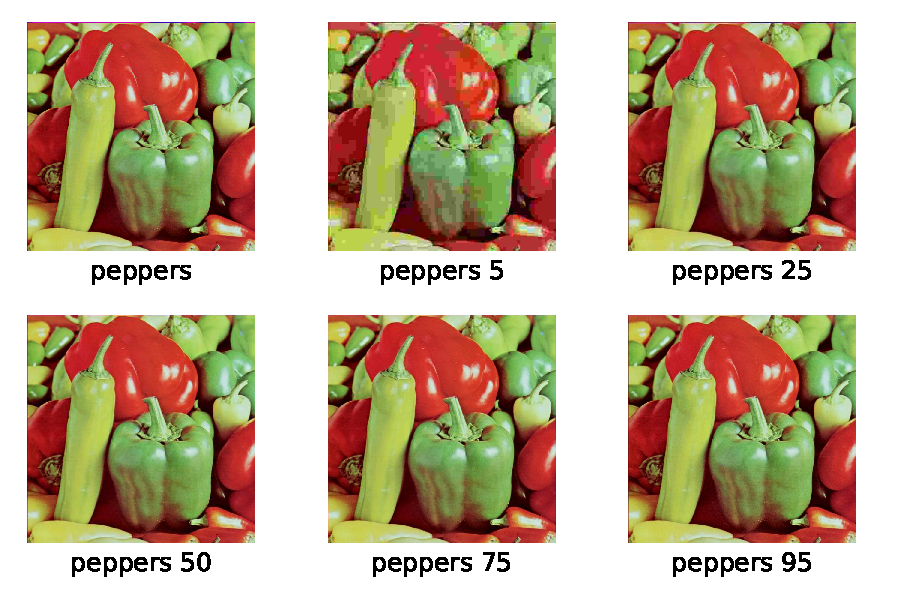
\includegraphics[width=1\textwidth]{slike/Quality_peppers.pdf}
\end{center}
\caption{Peppers prikazan v različnih kvalitetah. Levo zgoraj je original iz formata TIFF. Ostali so v formatu JPEG, kjer številka zraven imena predstavlja nivo kvalitete nastavljen v knjižnici PIL za generiranje JPEG-a. Vir: original~\cite{image_processing_slike} in ostale.}
\label{Quality_peppers}
\end{figure}

\begin{table}[ht]
\centering
    \begin{tabular}{|l|l|l|}
    \hline
    Ime slike in kvaliteta &PSNR   &velikost datoteke          \\
    \hline                   
    peppers original &$\infty$     & 769 kB                    \\ 
    peppers 5        & 19,90       & 8   kB                    \\
    peppers 25       & 23,50       & 17  kB                    \\  
    peppers 50       & 24,85       & 26  kB                    \\  
    peppers 75       & 26,21       & 41  kB                    \\  
    peppers 95       & 28,85       & 122 kB                    \\  
    \hline
    \end{tabular}
    \caption{Tabela z vrednostmi PSNR in velikostmi datoteke za različne kakovosti slike peppers. Prva vrstica tabele predstavlja original v formatu TIFF, ostale vrstice predstavljajo kompresirane slike v JPEG z kvaliteto, ki je zapisana v prvem stolpcu.}
\label{tab:peppers_psnr}
\end{table}

\begin{figure}[ht] % vir python
\begin{center}
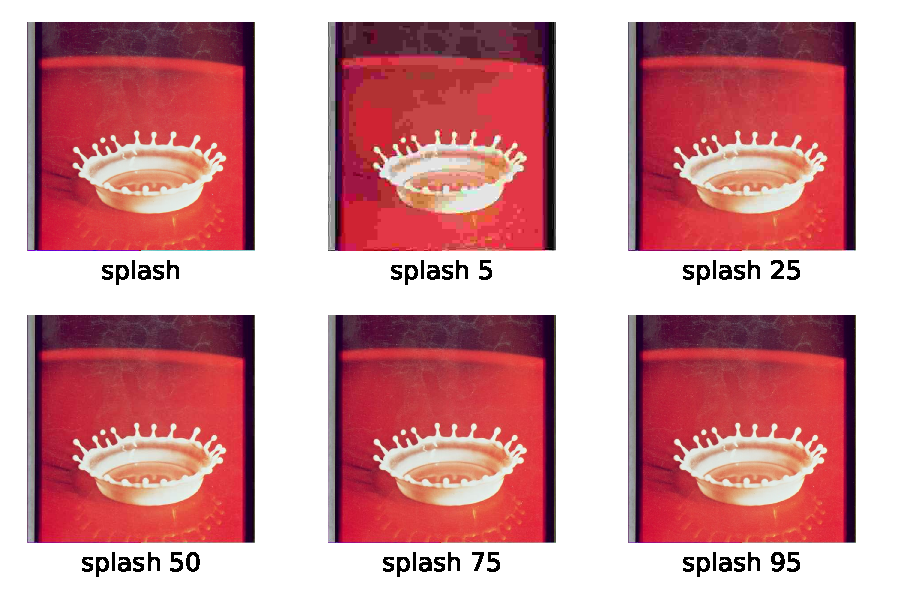
\includegraphics[width=1\textwidth]{slike/Quality_splash.pdf}
\end{center}
\caption{Splash prikazan v različnih kvalitetah. Levo zgoraj je original iz formata TIFF. Ostali so v formatu JPEG, kjer številka zraven imena predstavlja nivo kvalitete nastavljen v knjižnici PIL za generiranje JPEG-a. Vir: original~\cite{image_processing_slike} in ostale.}
\label{Quality_splash}
\end{figure}

\begin{table}[ht]
\centering
    \begin{tabular}{|l|l|l|}
    \hline
    Ime slike in kvaliteta &PSNR   &velikost datoteke         \\
    \hline                   
    splash original &$\infty$      & 769 kB                   \\ 
    splash 5        & 23,14        & 7   kB                   \\
    splash 25       & 28,04        & 13  kB                   \\  
    splash 50       & 29,25        & 20  kB                   \\  
    splash 75       & 30,29        & 32  kB                   \\  
    splash 95       & 32,07        & 88  kB                   \\  
    \hline
    \end{tabular}
    \caption{Tabela z vrednostmi PSNR in velikostmi datoteke za različne kakovosti slike splash. Prva vrstica tabele predstavlja original v formatu TIFF, ostale vrstice predstavljajo kompresirane slike v JPEG z kvaliteto, ki je zapisana v prvem stolpcu.}
\label{tab:splash_psnr}
\end{table}

\chapter{Sklepne ugotovitve}
Pokazali smo kako poteka kodiranje JPEG-a s pomočjo DCT. V tem procesu smo spoznali še veliko metod, ki so potrebne, da se to združi v celoto za kompresijo. Opisali smo sicer zgolj najbolj pogosto uporabljano verzijo JPEG-a. V samem standardu je še veliko specifik in pametnih idej, da ta format deluje tako dobro kot deluje. Sam format je bil zelo dobro zasnovan, saj se uporablja še 30 let po njegovem nastanku. Kljub temu, da so najmočnejši računalniki devetdesetih let enakovredni današnjim pametnim telefonom je ta format še vedno najbolj uporabljan. Obstajajo sicer že boljši formati, a zaradi svoje enostavnosti in efektivnosti ga ni nadomestil še nobeden. Vsak dan nastane več milijard slik v formatu JPEG in ta številka se le veča.\par
V \ref{Uporaba_DCT}. poglavju smo na nekaj primerih slik pogledali efektivnost kompresije z mero PSNR. Tukaj bi bilo zanimivo dodati še mero SSIM (\textit{angl.} structural similarity index measure), ki bolje upošteva zaznavanje človeškega očesa kot PSNR. PSNR gleda bolj matematično na razliko med dvema slikama, kar v praksi ni nujno tako dobro. 


%\cleardoublepage
%\addcontentsline{toc}{chapter}{Literatura}
\printbibliography[heading=bibintoc,title={Literatura}]
\end{document}







\begin{comment}
Izsek slike:
[[182 161 152 164 165 171 188 191]
 [160 157 169 176 179 177 181 189]
 [173 176 179 180 187 182 169 175]
 [190 186 183 176 182 184 169 164]
 [185 195 189 178 176 183 180 167]
 [185 190 189 185 177 175 177 170]
 [184 171 182 185 180 174 172 174]
 [175 186 179 178 180 182 181 184]]

 Izsek slike -128:
 [[54 33 24 36 37 43 60 63]
  [32 29 41 48 51 49 53 61]
  [45 48 51 52 59 54 41 47]
  [62 58 55 48 54 56 41 36]
  [57 67 61 50 48 55 52 39]
  [57 62 61 57 49 47 49 42]
  [56 43 54 57 52 46 44 46]
  [47 58 51 50 52 54 53 56]]

 DCT:
 [[399.1   3.5  -0.7   4.2   0.9   0.3   1.8   0. ]
 [-20.6 -27.3   9.3   6.1   9.8   2.3   1.1   1. ]
 [-15.1 -35.   15.4  -4.2  14.7   5.6  -3.1  -0.5]
 [ -2.7   3.8  15.3  -0.6  -0.9  12.   -5.2   0.3]
 [  3.4   4.7  16.6  10.   -8.9  -1.9  -4.   -2.8]
 [ -4.8  10.9   3.4   9.1  10.1   4.1   4.1   1.1]
 [  5.    5.7   3.9   0.3  -3.3  -4.4  -4.6  -2.5]
 [  0.2  -0.4  -0.    0.3  -0.2  -0.   -0.   -0.3]]

 DCT kvantizirano:
 [[25  0  0  0  0  0  0  0]
 [-2 -2  1  0  0  0  0  0]
 [-1 -3  1  0  0  0  0  0]
 [ 0  0  1  0  0  0  0  0]
 [ 0  0  0  0  0  0  0  0]
 [ 0  0  0  0  0  0  0  0]
 [ 0  0  0  0  0  0  0  0]
 [ 0  0  0  0  0  0  0  0]]

 dekvantiziramo:
 [[400   0   0   0   0   0   0   0]
  [-24 -24  14   0   0   0   0   0]
  [-14 -39  16   0   0   0   0   0]
  [  0   0  22   0   0   0   0   0]
  [  0   0   0   0   0   0   0   0]
  [  0   0   0   0   0   0   0   0]
  [  0   0   0   0   0   0   0   0]
  [  0   0   0   0   0   0   0   0]]

  Približek -128
[[40 36 31 30 36 47 60 69]
 [40 40 39 41 44 49 54 57]
 [44 47 51 53 53 50 46 44]
 [54 56 58 59 56 49 43 38]
 [62 61 59 56 52 48 44 42]
 [62 60 56 53 50 49 48 48]
 [54 54 53 53 53 52 51 51]
 [45 48 52 55 56 55 53 51]]

 Priblizek
[[168 164 159 158 164 175 188 197]
 [168 168 167 169 172 177 182 185]
 [172 175 179 181 181 178 174 172]
 [182 184 186 187 184 177 171 166]
 [190 189 187 184 180 176 172 170]
 [190 188 184 181 178 177 176 176]
 [182 182 181 181 181 180 179 179]
 [173 176 180 183 184 183 181 179]]

 Napaka
[[ 14  -3  -7   6   1  -4   0  -6]
 [ -8 -11   2   7   7   0  -1   4]
 [  1   1   0  -1   6   4  -5   3]
 [  8   2  -3 -11  -2   7  -2  -2]
 [ -5   6   2  -6  -4   7   8  -3]
 [ -5   2   5   4  -1  -2   1  -6]
 [  2 -11   1   4  -1  -6  -7  -5]
 [  2  10  -1  -5  -4  -1   0   5]]

 
\end{comment}